\documentclass[accepted]{uai2026} % camera-ready version
                        
%% There is a class option to choose the math font
% \documentclass[mathfont=ptmx]{uai2026} % ptmx math instead of Computer
                                         % Modern (has noticeable issues)
% \documentclass[mathfont=newtx]{uai2026} % newtx fonts (improves upon
                                          % ptmx; less tested, no support)
% NOTE: Only keep *one* line above as appropriate, as it will be replaced
%       automatically for papers to be published. Do not make any other
%       change above this note for an accepted version.

%% Choose your variant of English; be consistent
\usepackage[american]{babel}
% \usepackage[british]{babel}

%% Some suggested packages, as needed:
\usepackage{natbib} % has a nice set of citation styles and commands
    \bibliographystyle{plainnat}
    \renewcommand{\bibsection}{\subsubsection*{References}}
\usepackage{mathtools} % amsmath with fixes and additions
% \usepackage{siunitx} % for proper typesetting of numbers and units
\usepackage{booktabs} % commands to create good-looking tables
\usepackage{tikz} % nice language for creating drawings and diagrams

% --- Additional packages ---
\usepackage{amsfonts}
\usepackage{amssymb}
\usepackage{amsthm}
\usepackage{algorithm}
\usepackage{algorithmic}
\usepackage{xspace}
\usepackage{enumitem}
\usepackage{thmtools}
\usepackage{xcolor}
\usepackage{multirow}

% --- Theorem environments ---
\newtheorem{theorem}{Theorem}[section]
\newtheorem{lemma}[theorem]{Lemma}
\newtheorem{proposition}[theorem]{Proposition}
\newtheorem{corollary}[theorem]{Corollary}
\newtheorem{conjecture}[theorem]{Conjecture}
\theoremstyle{definition}
\newtheorem{definition}[theorem]{Definition}
\newtheorem{example}[theorem]{Example}
\theoremstyle{remark}
\newtheorem{remark}[theorem]{Remark}

% Custom macros
\newcommand{\AF}{\textsc{ApxFit}}
\newcommand{\VCdim}{\mathrm{VCdim}}
\newcommand{\disagree}{\mathrm{disagree}}
\newcommand{\poly}{\mathrm{poly}}
\DeclareMathOperator*{\argmin}{arg\,min}

%% Provided macros
% \smaller: Because the class footnote size is essentially LaTeX's \small,
%           redefining \footnotesize, we provide the original \footnotesize
%           using this macro.
%           (Use only sparingly, e.g., in drawings, as it is quite small.)

%% Self-defined macros

\title{When Can We Learn from Noisy Logical Data? Parameterized Complexity of Approximate Concept Fitting in Description Logics}

% The standard author block has changed for UAI 2026 to provide
% more space for long author lists and allow for complex affiliations
%
% All author information is authomatically removed by the class for the
% anonymous submission version of your paper, so you can already add your
% information below.
%
% Add authors
\author[1]{\href{mailto:chang.lu@yale.edu}{Chang~Lu}}
\author[2,3]{\href{mailto:zhaoyz@nju.edu.cn}{Yizheng~Zhao}\thanks{Corresponding author.}}
\author[4]{\href{mailto:renate.schmidt@manchester.ac.uk}{Renate~A.~Schmidt}}
\affil[1]{%
    Computational Biology and Biomedical Informatics Program\\
    Yale University\\
    New Haven, CT, USA
}
\affil[2]{%
    State Key Laboratory of Novel Software Technology\\
    Nanjing University\\
    Nanjing, China
}
\affil[3]{%
    School of Artificial Intelligence\\
    Nanjing University\\
    Nanjing, China
}
\affil[4]{%
    Department of Computer Science\\
    The University of Manchester\\
    Manchester, UK
}
  
  \begin{document}
\maketitle

%% ================================================================
%% ABSTRACT — changes marked in red
%% ================================================================
\begin{abstract}
  SAT-based bounded fitting (finding a smallest
  concept that correctly classifies all given examples) yields
  sample-efficient
  PAC learning for description
  logic (DL) concepts. Yet the paradigm is
  brittle: it demands ``\emph{realizability}'', and a single mislabeled
  example can render the SAT formula unsatisfiable. Learning
  without this assumption (\emph{agnostic} learning) is
  statistically possible for bounded-size classes; the real
  barrier is \emph{computational}: minimizing misclassifications
  over bounded-size concepts is NP-hard. We introduce
  $\AF(k,t)$, asking whether a DL concept of size at most~$k$
  misclassifies at most~$t$ examples, and chart the complexity
  landscape for
  fragments of the DL $\mathcal{ALC}$ whose operator
  sets contain conjunction and existential restriction
  ($\{\sqcap,\exists\}$) or, dually, $\{\sqcup,\forall\}$: the
  problem is \textbf{W[2]-hard} parameterized by~$k$
  (even for $t{=}0$), so its exponential cost
  cannot be confined to~$k$ alone, yet lies in \textbf{XP}
  parameterized by outlier
  count~$t$, that is, solvable in polynomial time
  for every fixed $(k,t)$. Algorithmically, we lift bounded
  fitting from SAT to MAX-SAT and combine it with structural risk
  minimization: the result satisfies an oracle inequality adapting
  to the unknown optimal size and noise rate, yielding the
  first noise-tolerant DL concept learner with formal agnostic
  generalization guarantees. On four ontology benchmarks, it retains
  accuracy $\geq 0.85$ under $10\%$ label noise, where exact
  fitting collapses to $0.45$ or below.
\end{abstract}

%% ================================================================
%% SECTION 1: INTRODUCTION
%% ================================================================
\section{Introduction}\label{sec:intro}

A central task in computational learning theory is to find, from
labeled examples, a concept that generalizes well to unseen
data~\citep{DBLP:journals/cacm/Valiant84}. When the concept class
consists of logical formulas, such as Boolean
formulas~\citep{DBLP:conf/stoc/KearnsLPV87,
DBLP:journals/jacm/PittV88}, decision
trees~\citep{DBLP:conf/aaai/GahlawatZ24}, first-order
definable concepts~\citep{DBLP:conf/lics/Bergerem19}, or description
logic (DL) concepts~\citep{DBLP:conf/colt/CohenH92,
DBLP:conf/ijcai/FunkJLPW19}, the search space is combinatorial, but
\emph{parsimony} serves as an inductive bias, formalized by
the Occam framework~\citep{DBLP:journals/jacm/BlumerEHW89,
DBLP:conf/stoc/BoardP90}: any algorithm
returning a \emph{consistent} concept (one fitting all
examples) whose size is polynomial in the target
size is a sample-efficient PAC learner. A natural instantiation is
\emph{bounded fitting}: search for a concept of size
$s = 1, 2, 3, \ldots$ that correctly classifies all examples, and
return the first one found. Inspired by bounded model
checking~\citep{DBLP:conf/tacas/BiereCCZ99},
\citet{DBLP:conf/ijcai/CateFJL23} realized this idea for DL concept
learning by encoding bounded fitting as propositional satisfiability
(SAT), obtaining the first provable PAC guarantees for DL concepts.
\citet{DBLP:conf/semweb/FunkJV25} extended this SAT-based approach
from lightweight DL $\mathcal{EL}$ to expressive
$\mathcal{ALC}$~\citep{DBLP:books/daglib/0041477}, establishing
NP-completeness of bounded fitting and developing efficient
encodings.

Bounded fitting, however, requires \emph{realizability}: a concept
of the given size must correctly classify \emph{every} example. A single mislabeled example renders the SAT formula
unsatisfiable,
forcing the algorithm to either fail or inflate the size bound until
the concept overfits the noise, a brittleness
that no solver engineering can remove.
Noise tolerance is a long-standing concern in learning
theory~\citep{DBLP:journals/ml/AngluinL87,
DBLP:journals/siamcomp/KearnsL93}, and existing DL concept learners
address it only implicitly, through fitness functions or approximate
matching: DL-Learner~\citep{DBLP:journals/ws/BuhmannLW16},
EvoLearner~\citep{DBLP:conf/www/HeindorfBDWGDN22},
DL-FOIL~\citep{DBLP:conf/ilp/FanizzidE08}, and neural
approaches~\citep{DBLP:conf/esws/KouagouHDN23} all lack formal
generalization guarantees under noise.
A principled remedy is already visible in the bounded-fitting
framework itself: \citet{DBLP:conf/ijcai/CateFJL23} note that
handling erroneous labels calls for admitting imperfect fittings,
where ``the optimization features of {SAT} solvers and Max-{SAT}
solvers seem to be promising'', and leave this as an open problem.
The same move has succeeded in neighboring settings, where MAX-SAT
handles noisy data for temporal logic
specifications~\citep{DBLP:conf/atva/GaglioneNRTX21} and
interpretable classification
rules~\citep{DBLP:conf/cp/MaliotovM18}.

Before committing to that route, it is worth
asking whether standard learning theory already settles the noise
problem.
Bounded-size DL concepts form a finite concept class
whose VC-dimension is $O(k\log|\Sigma|)$
(Proposition~\ref{prop:vcdim}), where $k$ is the concept
size and $|\Sigma|$ the signature size (the
number of available concept and role names). By the fundamental theorem
of statistical
learning~\citep{DBLP:books/daglib/0033642,
DBLP:journals/iandc/Haussler92}, every such class is agnostic PAC
learnable: the empirical risk minimizer (ERM),
the concept of size at
most~$k$ that minimizes classification error on the training
data, comes within
$O(\sqrt{k\log|\Sigma|/m})$ of the best-in-class risk, where $m$ is the sample
size~\citep{DBLP:journals/ml/KearnsSS94}. The barrier is therefore
not statistical but \emph{computational}: even the special case of
zero error (exact fitting, $t{=}0$) is
NP-complete~\citep{DBLP:conf/semweb/FunkJV25}, so computing the
ERM for arbitrary error levels cannot be easier. The
right question is then not \emph{whether} bounded-size DL concepts are
noise-tolerantly learnable, but \emph{for which parameterizations}
the intractable ERM computation becomes efficient.

Parameterized complexity~\citep{DBLP:series/txcs/DowneyF13,
DBLP:books/sp/CyganFKLMPPS15} is designed for
this question. Instead of a binary polynomial/NP-hard verdict, it asks
which \emph{parameters} confine a problem's exponential cost:
a problem is \emph{fixed-parameter tractable} (FPT) in
parameter~$\kappa$ if solvable in time $f(\kappa) \cdot n^{O(1)}$
on inputs of size~$n$,
and \emph{W-hard} if no such algorithm exists under standard
assumptions.
The framework speaks directly to learning.
\citet{DBLP:conf/aaai/BrandGS23} show, in the
realizable setting, that FPT consistency checking yields efficient
PAC learning. The closest precedent for our question is
\citet{DBLP:conf/aaai/GahlawatZ24}: for decision trees with
outliers, learning is W[1]-hard in tree size alone but FPT once the
outlier count (with the maximum example difference) joins the
parameter. We chart the analogous frontier for
DL concepts.
Although the complexity of DL concept
learning has been studied for three decades~\citep{DBLP:conf/colt/CohenH92,
DBLP:journals/ml/CohenH94}, from separability and
fitting~\citep{DBLP:conf/ijcai/FunkJLPW19, DBLP:conf/semweb/FunkJV25}
to active learning~\citep{DBLP:conf/ijcai/FunkJL21}, every such
result presupposes realizability. The parameterized complexity of
\emph{approximate fitting}, where a bounded-size concept may
disagree with some noisy examples, is uncharted, and it is where we
begin.

\paragraph{Contributions.} We make the following contributions:
\begin{enumerate}[leftmargin=*,itemsep=2pt,topsep=3pt]
  \item \textbf{Problem formulation.} We define
    $\AF(k,t)$: given labeled examples,
    does there exist a concept of size at most~$k$ that
    misclassifies at most~$t$ examples? This generalizes
    exact fitting ($t{=}0$) and directly captures the ERM
    computation underlying agnostic PAC learning
    (\S\ref{sec:problem}).

  \item \textbf{A complexity dichotomy.}
    For every fragment of
    $\mathcal{ALC}$ whose operator set~$O$ contains
    conjunction and existential restriction
    ($\{\sqcap, \exists\} \subseteq O$) or
    disjunction and universal restriction
    ($\{\sqcup, \forall\} \subseteq O$),    $\AF(k,t)$ is \textsf{W[2]-hard}
    parameterized by~$k$, even for exact fitting
    ($t{=}0$); yet, for any operator set and any fixed~$k$,
    $\AF(k,t)$ lies in XP parameterized    by outlier count~$t$, solvable in time
    $O(m^t \cdot p(N))$ for a polynomial~$p$ depending
    on~$k$, where $N$ is the input size. Concept size drives intractability, while outlier
    count restores tractability
    (\S\ref{sec:complexity}).

  \item \textbf{MAX-SAT algorithm with generalization guarantees.}
    We lift bounded fitting from SAT to partial weighted
    MAX-SAT, where hard clauses (which must all
    hold) enforce syntactic and semantic
    correctness and soft clauses (satisfied as many as possible)
    encode example classification, and
    combine it with structural risk
    minimization (SRM)~\citep{DBLP:conf/nips/Vapnik91}. The resulting
    algorithm is the first noise-tolerant DL concept learner with
    formal agnostic PAC guarantees, achieving the oracle inequality
    $R(\hat{C}) \leq \min_s \{R_s^* +
    O(\sqrt{s\log|\Sigma|/m})\}$, where
    $R(\hat{C})$ is the true risk of the returned concept
    and $R_s^*$ the best
    achievable risk at concept size~$s$
    (\S\ref{sec:algorithm}).

  \item \textbf{Experiments.} On four standard ontology benchmarks with injected
    label noise at rates $5$--$30\%$, our approach degrades
    gracefully while exact fitting fails entirely, and matches
    it in noise-free settings
    (\S\ref{sec:experiments}).
\end{enumerate}

%% ================================================================
%% SECTION 2: PRELIMINARIES
%% ================================================================
\section{Preliminaries}\label{sec:prelim}

\subsection{Description Logics}\label{sec:prelim:dl}

Let $N_C$, $N_R$, and $N_I$ be countably infinite, mutually disjoint sets of 
\emph{concept names}, \emph{role names}, and \emph{individual names}, respectively. A \emph{signature} is a pair
$\Sigma = (\Sigma_C, \Sigma_R)$ of finite
sets $\Sigma_C \subseteq N_C$ and $\Sigma_R \subseteq N_R$.
We write $|\Sigma|$ for $|\Sigma_C| + |\Sigma_R|$.
\emph{$\mathcal{ALC}$-concepts} over~$\Sigma$ are built by the
grammar
%
\[
  C,D \;::=\; \top \mid \bot \mid A
    \mid \neg C \mid C \sqcap D \mid C \sqcup D
    \mid \exists r.C \mid \forall r.C
\]
%
where $A \in \Sigma_C$ and $r \in \Sigma_R$.
The \emph{size} $\|C\|$ of a concept~$C$ is the number of
occurrences of concept names, role names, $\top$, and $\bot$ in~$C$.
For a set of operators
$O \subseteq \{\sqcap, \sqcup, \neg, \exists, \forall\}$, we write
$L(O)$ for the fragment of $\mathcal{ALC}$ that uses only the
operators in~$O$ together with $\top$, $\bot$, and concept names.
Thus $\mathcal{ALC} = L(\{\sqcap, \sqcup, \neg, \exists, \forall\})$,
and $\mathcal{EL} = L(\{\sqcap, \exists\})$.

An \emph{interpretation} is a pair
$\mathcal{I} = (\Delta^{\mathcal{I}}, {\cdot}^{\mathcal{I}})$
consisting of a non-empty \emph{domain} $\Delta^{\mathcal{I}}$ and a
function ${\cdot}^{\mathcal{I}}$ that maps every $A \in N_C$ to
$A^{\mathcal{I}} \subseteq \Delta^{\mathcal{I}}$, every $r \in N_R$
to $r^{\mathcal{I}} \subseteq \Delta^{\mathcal{I}} \times
\Delta^{\mathcal{I}}$, and every $a \in N_I$ to
$a^{\mathcal{I}} \in \Delta^{\mathcal{I}}$.
The \emph{extension} $C^{\mathcal{I}}$ of a concept~$C$ in
$\mathcal{I}$ is defined inductively:
$\top^{\mathcal{I}} = \Delta^{\mathcal{I}}$,
$\bot^{\mathcal{I}} = \emptyset$,
$(\neg C)^{\mathcal{I}} = \Delta^{\mathcal{I}} \setminus
C^{\mathcal{I}}$,
$(C \sqcap D)^{\mathcal{I}} = C^{\mathcal{I}} \cap
D^{\mathcal{I}}$,
$(C \sqcup D)^{\mathcal{I}} = C^{\mathcal{I}} \cup
D^{\mathcal{I}}$,
$(\exists r.C)^{\mathcal{I}} = \{ d \in \Delta^{\mathcal{I}} \mid
\exists e.\, (d,e) \in r^{\mathcal{I}} \wedge e \in
C^{\mathcal{I}}\}$, and
$(\forall r.C)^{\mathcal{I}} = \{ d \in \Delta^{\mathcal{I}} \mid
\forall e.\, (d,e) \in r^{\mathcal{I}} \rightarrow e \in
C^{\mathcal{I}}\}$.
We say that $d \in \Delta^{\mathcal{I}}$ \emph{satisfies}~$C$ in
$\mathcal{I}$ if $d \in C^{\mathcal{I}}$, and
call~$e$ an \emph{$r$-successor} of~$d$ in~$\mathcal{I}$ if
$(d,e) \in r^{\mathcal{I}}$.

A \emph{labeled example} is a triple $(\mathcal{I}, a, \ell)$ where
$\mathcal{I}$ is a finite interpretation (i.e.,
$\Delta^{\mathcal{I}}$ is finite), $a \in N_I$,
and $\ell \in \{+,-\}$.
An example is \emph{positive} if $\ell = +$ and \emph{negative} if
$\ell = -$. A labeled example is \emph{over}~$\Sigma$
if all symbols outside~$\Sigma$ have empty extensions
in~$\mathcal{I}$.
A concept~$C$ \emph{fits} a labeled example $(\mathcal{I}, a, +)$ if
$a^{\mathcal{I}} \in C^{\mathcal{I}}$, and fits
$(\mathcal{I}, a, -)$ if $a^{\mathcal{I}} \notin C^{\mathcal{I}}$.

\subsection{PAC Learning}\label{sec:prelim:pac}

We recall the agnostic PAC
model. Let $\mathcal{X}$ be an instance space
and let $\mathcal{H} \subseteq \{h : \mathcal{X} \to \{0,1\}\}$ be a
concept class. The \emph{true risk} of $h \in \mathcal{H}$ with
respect to a distribution $\mathcal{D}$ over
$\mathcal{X} \times \{0,1\}$ is
$R(h) = \Pr_{(x,y) \sim \mathcal{D}}[h(x) \neq y]$.
The \emph{empirical risk} on a sample
$S = ((x_1, y_1), \ldots, (x_m, y_m))$ is
$\hat{R}_S(h) = \frac{1}{m}\sum_{i=1}^{m} \mathbf{1}[h(x_i) \neq y_i]$,
where $\mathbf{1}[\cdot]$ denotes the indicator function.
The \emph{empirical risk minimizer} (ERM) over~$\mathcal{H}$ returns
$\hat{h} \in \argmin_{h \in \mathcal{H}} \hat{R}_S(h)$.

A concept class $\mathcal{H}$ is \emph{agnostic PAC learnable} if
there exists an algorithm that, for every $\epsilon, \delta > 0$ and
every distribution $\mathcal{D}$, given
$m = \text{poly}(1/\epsilon, 1/\delta)$ i.i.d.\ examples from
$\mathcal{D}$, returns $\hat{h}$ satisfying
$R(\hat{h}) \leq \min_{h \in \mathcal{H}} R(h) + \epsilon$
with probability at least $1-\delta$.
A finite concept class $\mathcal{H}$ satisfies this
guarantee via the ERM, with sample complexity
$m = O(\frac{1}{\epsilon^2}(\log|\mathcal{H}| +
\log(1/\delta)))$; more generally, learnability is governed by the
VC-dimension $\VCdim(\mathcal{H})$~\citep{DBLP:journals/jct/Sauer72,
DBLP:journals/jacm/BlumerEHW89}, which for finite classes is at
most $\log_2|\mathcal{H}|$.
For DL concept learning, the relevant concept class is
$\mathcal{H}_{k}^{L(O),\Sigma}$: the set of all $L(O)$-concepts
over $\Sigma$ of size at most~$k$, viewed as
classifiers on instances $(\mathcal{I}, a)$, mapping
$(\mathcal{I}, a)$ to $\mathbf{1}[a^{\mathcal{I}}
\in C^{\mathcal{I}}]$ (identifying label $+$ with $1$
and $-$ with $0$).
Since $|\mathcal{H}_{k}^{L(O),\Sigma}|$ is finite (bounded by
$|\Sigma|^{O(k)}$; see Appendix~\ref{app:vc}), the class is
agnostic PAC learnable with sample complexity
$O(\frac{k \log|\Sigma| + \log(1/\delta)}{\epsilon^2})$.

\subsection{Parameterized Complexity}\label{sec:prelim:param}

A \emph{parameterized problem} is a language
$\Pi \subseteq \{0,1\}^* \times \mathbb{N}$ where each instance
$(x, \kappa)$ consists of an input~$x$ and a
parameter~$\kappa \in \mathbb{N}$. The problem is
\emph{fixed-parameter tractable} (FPT) if there exists a computable
function~$f$ and a constant~$c$ such that $(x,\kappa) \in \Pi$ can be
decided in time $f(\kappa) \cdot |x|^c$. It is in the class
\emph{XP} if it can be decided in time $|x|^{f(\kappa)}$.
The \emph{W-hierarchy}
$\textsf{FPT} \subseteq \textsf{W[1]} \subseteq
\textsf{W[2]} \subseteq \cdots$
provides a sequence of presumably strict
inclusions~\citep{DBLP:series/txcs/DowneyF13}. Hardness for
$\textsf{W}[i]$ is established via \emph{parameterized reductions}
from a problem~$\Pi$ to a problem~$\Pi'$:
a function $(x, \kappa) \mapsto (x', \kappa')$ computable in FPT
time with $\kappa' \leq g(\kappa)$ for some computable~$g$,
such that $(x, \kappa) \in \Pi$ if and only if
$(x', \kappa') \in \Pi'$.

The canonical \textbf{W[2]}-complete problem,
from which our hardness proof in \S\ref{sec:complexity}
reduces, is \textsc{Hitting
Set}~\citep{DBLP:series/txcs/DowneyF13}: given a universe~$U$,
a family $\mathcal{F} \subseteq 2^U$, and
$\kappa \in \mathbb{N}$, decide whether there exists
$H \subseteq U$ with $|H| \leq \kappa$ such that
$H \cap F \neq \emptyset$ for every $F \in \mathcal{F}$.

%% ================================================================
%% SECTION 3: THE APXFIT PROBLEM
%% ================================================================
\section{The \AF{} Problem}\label{sec:problem}

The bounded fitting problem studied
by ten Cate et al.\ and Funk et al.\ asks whether some
concept of size at most~$k$ fits \emph{all} given examples, a
requirement that, as \S\ref{sec:intro} argued, is brittle
under label noise. We generalize it by allowing a bounded number
of misclassified examples.

\begin{definition}\label{def:disagree}  Let $E = \{(\mathcal{I}_1, a_1, \ell_1), \ldots,
  (\mathcal{I}_m, a_m, \ell_m)\}$ be a set of labeled examples,
  let~$C$ be a concept, and write $[m]$ for
  $\{1, \ldots, m\}$. The \emph{disagreement} of~$C$ on~$E$ is
  %
  \begin{multline*}
    \textnormal{disagree}(C, E) =
    \bigl|\{ i \in [m] : \ell_i{=}{+},\,
      a_i^{\mathcal{I}_i} \notin C^{\mathcal{I}_i} \}\bigr|
    \\    +\;
    \bigl|\{ i \in [m] : \ell_i{=}{-},\,
      a_i^{\mathcal{I}_i} \in C^{\mathcal{I}_i} \}\bigr|,
  \end{multline*}
  %
  i.e., the number of false negatives plus false positives.
\end{definition}

\begin{definition}\label{def:apxfit}
  Fix an operator set
  $O \subseteq \{\sqcap, \sqcup, \neg, \exists, \forall\}$ and a
  signature~$\Sigma$. The problem $\AF(k,t)$ is: given a set~$E$ of
  labeled examples over~$\Sigma$ and parameters
  $k, t \in \mathbb{N}$, decide whether there exists an
  $L(O)$-concept~$C$ over~$\Sigma$ with $\|C\| \leq k$ and
  $\textnormal{disagree}(C, E) \leq t$.
\end{definition}

Setting $t = 0$ recovers the exact fitting problem of
\citet{DBLP:conf/semweb/FunkJV25}, which is NP-complete for every
$O$ with $O \cap \{\exists, \forall\} \neq \emptyset$.
The optimization version
$\min_{\|C\| \leq k} \textnormal{disagree}(C, E)$ is precisely
the ERM computation over the concept class
$\mathcal{H}_{k}^{L(O),\Sigma}$ defined in
\S\ref{sec:prelim:pac}: viewing~$E$ as
the sample~$S$, the empirical risk $\hat{R}_S(C)$
equals $\textnormal{disagree}(C, E) / m$. The problem $\AF(k,t)$
thus captures the decision version of agnostic concept learning,
parameterized by concept size~$k$ and outlier count~$t$.

\begin{proposition}[Statistical--computational
separation]\label{prop:separation}
  Let $O \subseteq \{\sqcap, \sqcup, \neg, \exists, \forall\}$ with
  $O \cap \{\exists, \forall\} \neq \emptyset$. (i) \textnormal{(Statistical)} The concept class
      $\mathcal{H}_{k}^{L(O),\Sigma}$ is agnostic PAC learnable
      with sample complexity
      $O\bigl(\frac{k \log|\Sigma| + \log(1/\delta)}{\epsilon^2}\bigr)$,
      where the cardinality term $k \log|\Sigma|$ is tight up to
      constant factors
      (Appendix~\ref{app:vc}, Remark~\ref{rem:tight});
      (ii) \textnormal{(Computational)} $\AF(k,t)$ is
      \textnormal{NP}-complete, even for fixed $t = 0$.
\end{proposition}
\begin{proof}[Proof sketch
  (full proof in Appendix~\ref{app:sep-proof})]
  (i) follows from finiteness of
  $\mathcal{H}_{k}^{L(O),\Sigma}$ via the finite-class bound
  (\S\ref{sec:prelim:pac}). For~(ii), membership holds
  because a concept of size at most~$k$ can be guessed and
  evaluated on all $m$ examples in polynomial time; hardness is
  immediate from the $t = 0$ case, which is NP-complete as noted
  above.
\end{proof}

Proposition~\ref{prop:separation} formalizes
the statistical--computational gap previewed in
\S\ref{sec:intro}.

%% ================================================================
%% SECTION 4: PARAMETERIZED COMPLEXITY RESULTS (NEW)
%% ================================================================
\section{Parameterized Complexity}\label{sec:complexity}

We now refine the classical NP-completeness of
Proposition~\ref{prop:separation} through two natural
parameterizations: concept size~$k$ and outlier count~$t$.

\subsection{Intractability by Concept Size}\label{sec:complexity:hard}

The NP-hardness proof
of Funk et al.\ for exact fitting reduces
from \textsc{Hitting Set}, but the resulting concept size grows with
the input. We give a different reduction in which the concept
size depends \emph{only} on the hitting set parameter~$\kappa$,
establishing W[2]-hardness. The key idea is to encode universe
elements as role names in the signature (which
is part of the input) rather than as positions inside the concept.

\begin{theorem}[{W[2]-hardness}]\label{thm:w2hard}
  $\AF(k,t)$ is \textsf{W[2]}-hard parameterized
  by~$k$, for every operator set~$O$ with
  $\{\sqcap, \exists\} \subseteq O$ or
  $\{\sqcup, \forall\} \subseteq O$.
  Hardness holds even for $t = 0$ and with
  $\Sigma_C = \emptyset$.
\end{theorem}

\begin{proof}[Proof sketch
  (full proof in Appendix~\ref{app:w2hard})]
  We present the case
  $\{\sqcap, \exists\} \subseteq O$; the dual case follows by
  exchanging $\sqcap \leftrightarrow \sqcup$,
  $\exists \leftrightarrow \forall$, and swapping positive and
  negative labels. Given a \textsc{Hitting Set} instance
  $(U, \mathcal{F}, \kappa)$ with $U = \{u_1, \ldots, u_n\}$ and
  $\mathcal{F} = \{F_1, \ldots, F_v\}$, we construct an
  $\AF(k, 0)$ instance over the signature
  $\Sigma_C = \emptyset$,
  $\Sigma_R = \{r_1, \ldots, r_n\}$, with $k = 2\kappa$.
  The single positive example $(\mathcal{I}^+, a, +)$ has $a$
  connected via each~$r_i$ to a dead-end element~$d$ (no outgoing
  roles, no concept names). For each $F_j \in \mathcal{F}$, the
  negative example $(\mathcal{I}_j, b_j, -)$ has $b_j$ connected
  via~$r_i$ to a dead-end~$d_j$ only for $i \notin F_j$
  (Example~\ref{ex:reduction} illustrates the
  construction).

  \emph{Forward.} A hitting set
  $H = \{u_{i_1}, \ldots, u_{i_q}\}$ yields
  $C = \exists r_{i_1}.\top \sqcap \cdots \sqcap
  \exists r_{i_q}.\top$ with $\|C\| = 2q \leq 2\kappa$.
  The element~$a$ satisfies every conjunct (all $r_i$-successors
  exist). Each~$b_j$ fails some conjunct since
  $H \cap F_j \neq \emptyset$ implies some $r_{i_h}$-successor
  is absent.

  \emph{Reverse.}
  Let $C$ be any $\mathcal{ALC}$-concept with $\|C\| \leq 2\kappa$
  fitting all examples. Since every element
  other than the roots $a$ and~$b_j$ is a dead end,
  any subconcept evaluates to a fixed Boolean constant on these
  elements. Consequently, the only subconcepts that
  distinguish~$a$ from some~$b_j$ are those of the form
  $\exists r_i.D$ with $D$
  true on dead ends, or dually $\forall r_i.D$ with $D$ false on
  dead ends; every other subconcept evaluates identically at the
  roots. Each occurrence of a role name in~$C$ costs at
  least~$2$ in concept size (the role name itself plus at least
  one symbol in its filler), so at most~$\kappa$ distinct role
  indices appear in~$C$. Setting
  $H = \{u_i : r_i \text{ occurs in } C\}$ gives
  $|H| \leq \kappa$. If $F_j \cap H = \emptyset$ for some~$j$,
  then $a$ and $b_j$ agree on all role names in~$C$, so $C$
cannot distinguish them, contradicting
$a \in C^{\mathcal{I}^+}$ and
  $b_j \notin C^{\mathcal{I}_j}$.\qedhere
\end{proof}

Two aspects merit comment: (i) the W[2]-hardness (as opposed to W[1]-hardness) reflects
the combinatorial structure of \textsc{Hitting Set} and the
ability of DL concepts to express arbitrary conjunctions of
existential restrictions, each selecting one element.
For comparison, Gahlawat and Zehavi obtain only
W[1]-hardness for decision trees via a reduction from
\textsc{Partial Vertex Cover}; (ii) Our fragment condition, requiring both
conjunction and
existential restriction (or dually, disjunction and universal
restriction), is necessary for the reduction. Whether
W-hardness holds for smaller fragments such as
$L(\{\exists\})$ remains open.

\begin{example}\label{ex:reduction}
  Consider the \textsc{Hitting Set} instance with
  universe $U = \{u_1, u_2, u_3\}$, family
  $\mathcal{F} = \{F_1, F_2\}$ where $F_1 = \{u_1, u_2\}$ and
  $F_2 = \{u_2, u_3\}$, and parameter $\kappa = 1$.
  The reduction produces the signature
  $\Sigma_R = \{r_1, r_2, r_3\}$ (no concept names) and the
  parameter $k = 2\kappa = 2$.

  The positive example $(\mathcal{I}^+, a, +)$ has
  domain $\{a, d\}$, with $r_1, r_2, r_3$ each mapping $(a, d)$;
  so $a$ has an $r_i$-successor for every $i$.
  Negative example $(\mathcal{I}_1, b_1, -)$ for
  $F_1 = \{u_1, u_2\}$ has domain $\{b_1, d_1\}$ with only
  $r_3^{\mathcal{I}_1} = \{(b_1, d_1)\}$; the roles $r_1, r_2$
  are empty (their indices are in~$F_1$).
  Similarly, $(\mathcal{I}_2, b_2, -)$ for $F_2 = \{u_2, u_3\}$
  has only $r_1^{\mathcal{I}_2} = \{(b_2, d_2)\}$.

  \emph{Forward}: the hitting set
  $H = \{u_2\}$ (size $1 \leq \kappa$) yields concept
  $C = \exists r_2.\top$ with $\|C\| = 2 \leq k$. Indeed,
  $a \in C^{\mathcal{I}^+}$ since $a$ has an $r_2$-successor;
  $b_1 \notin C^{\mathcal{I}_1}$ since $r_2^{\mathcal{I}_1}
  = \emptyset$ ($2 \in F_1$); and
  $b_2 \notin C^{\mathcal{I}_2}$ since
  $r_2^{\mathcal{I}_2} = \emptyset$ ($2 \in F_2$).

  \emph{Reverse}: any concept of size $\leq 2$
  that fits all examples can use at most one role name. If that
  role name is $r_i$, then $\{u_i\}$ must hit both $F_1$ and
  $F_2$, which forces $i = 2$, the unique element in
  $F_1 \cap F_2$. A concept using $r_1$ alone would fail on
  $b_2$ (which has an $r_1$-successor), and $r_3$ alone would fail
  on $b_1$ (which has an $r_3$-successor).
\end{example}

\paragraph{Relevance to learnability.}
One might object that hardness of \emph{exact} size minimization
says little about learning, since a learner need only find a
concept that generalizes, not one of provably minimal size.
Two considerations show that the barrier is genuine.
First, \citet{DBLP:conf/aaai/BrandGS23} show
that, under mild sampleability conditions, fixed-parameter PAC
learnability holds \emph{if and only if} the associated consistency-checking problem is
FPT (their Theorems~3.17 and~3.19). $\AF(k,0)$ is precisely this
consistency-checking problem for the class
$\mathcal{H}_k^{L(O),\Sigma}$, and our W[2]-hardness holds already
at $t = 0$; by the contrapositive of their Theorem~3.17, FPT-time PAC
learning parameterized by concept size is ruled out, independently
of any particular algorithm.
Second, relaxing exactness does not restore tractability: our
reduction is from \textsc{Hitting Set}, the
dual of \textsc{Set Cover} (the same problem with the roles of
sets and elements exchanged, so the two are equivalent under
parameterized reductions), and \citet{DBLP:conf/soda/LinRSW23} show that
approximating $k$-\textsc{Set Cover} within \emph{any} constant
factor is itself W[2]-hard. A constant-factor approximation of the
minimum concept size would therefore still be intractable when
parameterized by~$k$. The route to tractable learning must
instead pass through a different parameter.

\subsection{Tractability by Outlier Count}\label{sec:complexity:xp}

We now turn to the second parameter, the
outlier count~$t$.

\begin{theorem}[XP membership]\label{thm:xp}  For any fixed $k \in \mathbb{N}$ and any operator
  set~$O \subseteq \{\sqcap, \sqcup, \neg,
  \exists, \forall\}$, $\AF(k,t)$ parameterized by~$t$ is in
  \textnormal{XP}: it can be solved in time
  $O(m^t \cdot p(N))$, where $m$
  is the number of examples, $N$ the total input size, and $p$ is a polynomial whose
  degree depends on~$k$.
\end{theorem}

\begin{proof}[Proof sketch
  (full proof in Appendix~\ref{app:xp-proof})]
  Enumerate all
  $\sum_{i=0}^{t}\binom{m}{i} \leq (t{+}1)\, m^t$ subsets
  $T \subseteq E$ of size at most~$t$ and, for each~$T$, check
  exact fitting on $E \setminus T$ with size bound~$k$ by
  enumerating all
  $(c|\Sigma|)^k$ candidate concepts of size at
  most~$k$ (Lemma~\ref{lem:class-size}). Soundness and
  completeness are immediate; for fixed~$k$, each check costs
  time polynomial in the input size~$N$.
\end{proof}

\subsection{Summary}\label{sec:complexity:summary}

Table~\ref{tab:complexity} summarizes the
resulting complexity landscape.
The joint parameterization by
$(k, t)$ inherits W[2]-hardness directly from
Theorem~\ref{thm:w2hard}: the reduction produces instances with
$t = 0$, so the combined parameter $k + t = 2\kappa$ is bounded in
the \textsc{Hitting Set} parameter. This rules out algorithms
running in time $f(k,t) \cdot \poly(N)$ under standard
assumptions; it leaves open whether, for each fixed~$k$, the XP
running time of Theorem~\ref{thm:xp} can be improved to
$f(t) \cdot \poly(N)$.
Two further cells complete the picture.
Parameterized by~$k$ alone, the problem lies in XP: for
fixed~$k$, all $(c|\Sigma|)^k$ candidate concepts
(Corollary~\ref{cor:log-class}) can be enumerated and evaluated
in polynomial time, so under standard assumptions the
$k$-parameterization sits strictly between FPT and XP.
Parameterized by~$t$ alone, even XP membership fails unless
P${}={}$NP, since the slice $t = 0$ is already NP-complete
(Proposition~\ref{prop:separation}); this is why
Theorem~\ref{thm:xp} fixes~$k$.
This landscape parallels the decision-tree
results of \citet{DBLP:conf/aaai/GahlawatZ24}: our hardness is
stronger (W[2] versus their W[1]), while our tractability is
currently weaker (XP versus their FPT); closing the latter gap is
a natural direction for future work.
In the worst case, the XP exponent grows
with~$t$, so the enumeration is practical only for small outlier
counts.

\begin{table}[ht]
  \centering
  \caption{Parameterized complexity of $\AF(k,t)$.
  Hardness entries assume
  $\{\sqcap, \exists\} \subseteq O$ or
  $\{\sqcup, \forall\} \subseteq O$; membership entries hold for
  every operator set.}\label{tab:complexity}
  \small
  % camera-ready fix: table resized to exactly \columnwidth
  \resizebox{\columnwidth}{!}{%
  \begin{tabular}{@{}lll@{}}
    \toprule
    \textbf{Parameter} & \textbf{Complexity} & \textbf{Reference} \\
    \midrule
    $k$ (concept size) & W[2]-hard; in XP & Thm.~\ref{thm:w2hard} \\
    $t$ (outlier count) & not in XP unless P${}={}$NP & Prop.~\ref{prop:separation} ($t{=}0$) \\
    $t$ (outlier count), $k$ fixed & in XP; FPT open & Thm.~\ref{thm:xp} \\
    $(k, t)$ jointly & W[2]-hard & Thm.~\ref{thm:w2hard} ($t{=}0$) \\
    \bottomrule
  \end{tabular}%
  }
\end{table}

%% ================================================================
%% REMAINING SECTIONS (PLACEHOLDERS)
%% ================================================================
\section{MAX-SAT Algorithm with Structural Risk Minimization}\label{sec:algorithm}

The complexity results of \S\ref{sec:complexity} directly
shape the algorithm design. Theorem~\ref{thm:w2hard} rules out
uniformly efficient ERM computation in the concept size~$k$; we
therefore delegate each per-size ERM call to a MAX-SAT solver.
Since the optimal concept size is unknown a priori, the algorithm
iterates over candidate sizes $s = 1, \ldots, s_{\max}$ and
selects among the solutions using a complexity penalty.
The penalty derives from the concept
class cardinality bound (Appendix~\ref{app:vc}).
The XP algorithm of Theorem~\ref{thm:xp} shows
that $\AF(k,t)$ is solvable in polynomial time for each fixed~$t$,
but its $\binom{m}{t}$ enumeration is impractical for moderate
outlier counts. We therefore take a direct approach: encoding approximate fitting as
partial weighted MAX-SAT, and combining it with
SRM to obtain formal generalization
guarantees.

\subsection{Partial Weighted MAX-SAT Encoding}\label{sec:algorithm:maxsat}

Recall the SAT encoding of
\citet{DBLP:conf/semweb/FunkJV25} constructs, for a given size
bound~$k$ and example set~$E$, a propositional formula
$\Phi(k, E)$ whose satisfying assignments correspond to
$L(O)$-concepts~$C$ with $\|C\| \leq k$ and
$\disagree(C, E) = 0$. We refer to their
work for the full construction and
recall here only the high-level structure needed for our extension.

The clauses in $\Phi(k, E)$ decompose into two
groups:
%
\begin{itemize}[leftmargin=*,itemsep=1pt,topsep=2pt]
  \item \emph{Structural clauses} $\Phi_{\mathrm{struct}}(k)$:
    enforce that the propositional variables encode a valid
    $L(O)$-concept of size at most~$k$. These are independent of
    the examples.
  \item \emph{Classification clauses}
    $\phi_1(k), \ldots, \phi_m(k)$: one conjunction of clauses per
    example, where $\phi_i(k)$ is satisfiable together with
    $\Phi_{\mathrm{struct}}(k)$ if and only if the encoded concept
    correctly classifies example~$i$.
\end{itemize}

A \emph{partial weighted MAX-SAT} instance
consists of \emph{hard} clauses, which every solution must
satisfy, and weighted \emph{soft} clauses; an optimal solution
maximizes the total weight of satisfied soft clauses.

\begin{definition}[MAX-SAT encoding]\label{def:maxsat}
  Given a size bound~$k$ and example set $E$ of
  size~$m$, the \emph{partial weighted MAX-SAT instance}
  $\Psi(k, E)$ is obtained as follows. For
  each example $i \in [m]$, introduce a fresh relaxation
  variable~$z_i$.
  %
  \begin{itemize}[leftmargin=*,itemsep=1pt,topsep=2pt]
    \item \emph{Hard clauses}: all clauses in
      $\Phi_{\mathrm{struct}}(k)$,
      together with every clause of
      $\phi_i(k)$ augmented by the literal~$z_i$ (that is,
      $c \vee z_i$ for each clause $c \in \phi_i(k)$), for all
      $i \in [m]$;
    \item \emph{Soft clauses}: the unit
      clause $(\neg z_i)$ with weight~$1$, for each $i \in [m]$.
  \end{itemize}
  %
  Setting $z_i$ to true relaxes all
  classification constraints of example~$i$ at a cost of exactly
  one, independently of how many clauses of $\phi_i(k)$ the
  encoded concept violates.
\end{definition}

By construction (Proposition~\ref{prop:maxsat-correct},
Appendix~\ref{app:maxsat-correct}), an optimal solution to
$\Psi(k, E)$ encodes a concept $\hat{C}_k$ that minimizes
$\disagree(\hat{C}_k, E)$ over all $L(O)$-concepts of size at
most~$k$; that is, $\hat{C}_k$ is an ERM over $\mathcal{H}_{k}^{L(O),\Sigma}$. When all soft
clauses can be satisfied, the encoding reduces to the
exact fitting formulation of Funk et al.
The encoding size is polynomial in~$k$, $|\Sigma|$, and~$m$:
following Funk et al., 
the formula uses $O(k^2 + k|\Sigma| + k \cdot \|E\|)$ propositional
variables and $O(\|E\| \cdot k^3 \cdot |\Sigma|)$ clauses, where $\|E\|$
is the total size of all interpretations in~$E$; the relaxation
variables add only $m$ further variables and $m$ soft clauses.

\subsection{Structural Risk Minimization}\label{sec:algorithm:srm}

The ERM $\hat{C}_k$ for a single size bound~$k$
achieves the lowest training error in $\mathcal{H}_k$, but the
optimal concept size is unknown a priori;
henceforth we write~$s$ for the candidate size being iterated,
reserving~$k$ for the problem parameter. A small~$k$ may underfit,
while a large~$k$ may overfit noise. SRM resolves this by penalizing
complexity: it selects the size that best balances empirical fit
against a complexity-dependent penalty.

For each candidate size $s \in \{1, \ldots, s_{\max}\}$,
the uniform convergence bound for $\mathcal{H}_s =
\mathcal{H}_{s}^{L(O),\Sigma}$ guarantees that,
for a sample~$S$ of $m$ examples drawn i.i.d.\
from~$\mathcal{D}$, with probability at
least $1 - \delta'$,
\begin{equation}\label{eq:uc}
  \sup_{C \in \mathcal{H}_s}
    \bigl| \hat{R}_S(C) - R(C) \bigr|
  \;\leq\;
  \sqrt{\frac{2\bigl(s \log|\Sigma| + \log(2/\delta')\bigr)}{m}},
\end{equation}
using $\log |\mathcal{H}_s| \leq s \log |\Sigma| + O(s)$
(Appendix~\ref{app:vc}); the full derivation,
including the absorption of the $O(s)$ term, is in
Appendix~\ref{app:penalty}.

\begin{algorithm}[t]
  \caption{SRM-MaxSAT}\label{alg:srm}
  \begin{algorithmic}[1]    \REQUIRE Examples $E$ ($|E| = m$), maximum
      candidate size $s_{\max}$,
      failure probability $\delta \in (0,1)$    \ENSURE Concept $\hat{C}_{s^*}$ satisfying the
      oracle inequality (Theorem~\ref{thm:oracle})
    \FOR{$s = 1, 2, \ldots, s_{\max}$}
      \STATE $\hat{C}_s \leftarrow
        \text{MAX-SAT-Solve}(\Psi(s, E))$
        \hfill\COMMENT{ERM for $\mathcal{H}_s$}      \STATE $\hat{R}_s \leftarrow
        \disagree(\hat{C}_s, E) \,/\, m$
        \hfill\COMMENT{empirical risk}
      \STATE $\mathrm{pen}_s \leftarrow
        \sqrt{\frac{2\bigl(s \log|\Sigma| +        \log(2 s_{\max}/\delta)\bigr)}{m}}$
        \hfill\COMMENT{penalty from~\eqref{eq:uc}}
      \STATE $\mathrm{score}_s \leftarrow
        \hat{R}_s + \mathrm{pen}_s$
    \ENDFOR    \STATE $s^* \leftarrow
      \argmin_{s \in [s_{\max}]} \mathrm{score}_s$
      \hfill\COMMENT{SRM model selection}
    \RETURN $\hat{C}_{s^*}$
  \end{algorithmic}
\end{algorithm}

The penalty
$\mathrm{pen}_s$ in Algorithm~\ref{alg:srm} applies a union bound
correction
$\log(2 s_{\max}/\delta)$ to ensure simultaneous validity across
all $s_{\max}$ size classes. In practice,
early termination is possible once $\mathrm{pen}_s$ alone exceeds
the best score found so far: since $\mathrm{pen}_s$ is increasing
in~$s$ and $\mathrm{score}_{s'} \geq \mathrm{pen}_{s'} \geq
\mathrm{pen}_s$ for all $s' \geq s$, no larger size class can
attain a lower score.

\subsection{Generalization Guarantee}\label{sec:algorithm:guarantee}

\begin{theorem}[Oracle inequality]\label{thm:oracle}
  Let $\hat{C}$ be the output of
  Algorithm~\ref{alg:srm} on $m$ i.i.d.\ examples.
  For any $\delta \in (0,1)$, with probability at least
  $1 - \delta$:
  %
  \begin{equation}\label{eq:oracle}
    R(\hat{C}) \;\leq\;
    \min_{1 \leq s \leq s_{\max}} \biggl\{
      R_s^* + 2\sqrt{\frac{2\bigl(s \log|\Sigma| +
      \log\frac{2 s_{\max}}{\delta}\bigr)}{m}}
    \biggr\}
  \end{equation}
  %
  where $R_s^* = \inf_{C \in \mathcal{H}_s} R(C)$ is the optimal
  true risk achievable by concepts of size at most~$s$.
\end{theorem}

\begin{proof}[Proof sketch
  (full proof in Appendix~\ref{app:oracle})]
  Apply the uniform convergence
  bound~\eqref{eq:uc} to each of the
  $s_{\max}$ classes $\mathcal{H}_s$ with failure
  probability $\delta/s_{\max}$, and take a union bound over
  $s = 1, \ldots, s_{\max}$. With probability at least
  $1 - \delta$, for every $s$ and every $C \in \mathcal{H}_s$,
  $|R(C) - \hat{R}_S(C)| \leq \mathrm{pen}_s$.
  Since $\hat{C}_s$ is the ERM for $\mathcal{H}_s$
  (note $\hat{R}_s = \hat{R}_S(\hat{C}_s)$) and
  Algorithm~\ref{alg:srm} selects
  $s^* = \argmin_s (\hat{R}_s + \mathrm{pen}_s)$,
  standard SRM analysis yields~\eqref{eq:oracle}.
\end{proof}

The bound~\eqref{eq:oracle} is an oracle
inequality: without knowing the optimal concept size or noise
level, the algorithm automatically adapts to the best trade-off
between approximation error ($R_s^*$, decreasing in~$s$)
and estimation error ($\mathrm{pen}_s$, increasing in~$s$).
When the minimum in~\eqref{eq:oracle} is attained at size~$s^*$,
the excess risk $R(\hat{C}) - R^*_{s^*}$
is $O(\sqrt{s^* \log|\Sigma| / m})$, matching
the rate previewed in \S\ref{sec:intro}.
We emphasize that this is stronger than a standard PAC bound for a
fixed hypothesis class, which would indeed follow immediately from
uniform convergence once the class is fixed. The content
of~\eqref{eq:oracle} is that the \emph{data-dependent} choice of
size~$s^*$ competes with the best size in hindsight, over a nested
hierarchy $\mathcal{H}_1 \subseteq \cdots \subseteq
\mathcal{H}_{s_{\max}}$.
This model-selection guarantee is what the
exact bounded-fitting approaches of ten Cate et al.\ and
Funk et al.\ do not provide, since they fix
a single target size per invocation.

\subsection{Discussion}\label{sec:algorithm:discussion}

\emph{Relation to prior SAT-based approaches.}
Setting $s_{\max} = k$ and accepting only solutions with
$\disagree = 0$ reduces Algorithm~\ref{alg:srm} to the
iterative bounded fitting of ten Cate et al.: try size
$s = 1, 2, \ldots$ until the SAT formula is satisfiable.
The MAX-SAT encoding reuses the
structural clauses of Funk et al.\ without
modification; the classification clauses are retained as hard
clauses augmented with per-example relaxation variables, and one
soft unit clause per example replaces the requirement that every
example be classified correctly (Definition~\ref{def:maxsat}).

\emph{Comparison with adjacent work.}
MAX-SAT-based learning was explored for temporal logic
specifications~\citep{DBLP:conf/atva/GaglioneNRTX21} and
interpretable classification
rules~\citep{DBLP:conf/cp/MaliotovM18}, but without formal
PAC-style generalization guarantees. Reusing
the encoding of Funk et al.\ is a feature,
not a limitation: it isolates our contribution to the
size-selection layer: the combination of
MAX-SAT for per-size ERM with SRM for model selection, and the
resulting oracle inequality (Theorem~\ref{thm:oracle}), appears to
be new for DL concept learning.

\emph{Encoding versus problem hardness.}
The MAX-SAT encoding is a solution technique, not
the source of intractability: the W[2]-hardness of
Theorem~\ref{thm:w2hard} is a property of $\AF(k,t)$ itself and
holds for any algorithm. The encoding transfers this inherent
hardness to a solver whose conflict-driven search performs well
on structured instances, which our runtime
results confirm.

\emph{Scalability and relaxations.}
Two properties of the MAX-SAT formulation mitigate the
worst-case exponential cost in practice. First, MAX-SAT solvers can
be run in anytime configurations: in linear (model-improving)
search, interrupting the solver returns the best concept found so
far, and core-guided or hybrid configurations additionally
maintain a lower bound on the optimum, yielding an explicit
optimality gap. A suboptimal ERM enters the oracle inequality
only as an additive term, so the guarantee degrades gracefully
rather than failing. Second, the optimization itself admits
relaxations, such as solving to a target disagreement gap rather
than to optimality,
which trades a controlled additive term in the empirical risk
for solver time. Exploring such relaxed variants, as well as
probabilistic approaches that attach confidence values to learned
expressions~\citep{DBLP:journals/ml/LehmannH10}, is a promising
avenue for scaling beyond the benchmark sizes considered here.

\section{Experiments}\label{sec:experiments}

We evaluate SRM-MaxSAT (Algorithm~\ref{alg:srm})
against state-of-the-art baselines on standard benchmarks under varying label noise,
investigating three questions: (\textbf{Q1})~Does our approach degrade
gracefully under noise while exact fitting fails? (\textbf{Q2})~Does SRM
select appropriate concept sizes? (\textbf{Q3})~What is the runtime overhead
of MAX-SAT over SAT?

\begin{figure*}[t]
  \centering
  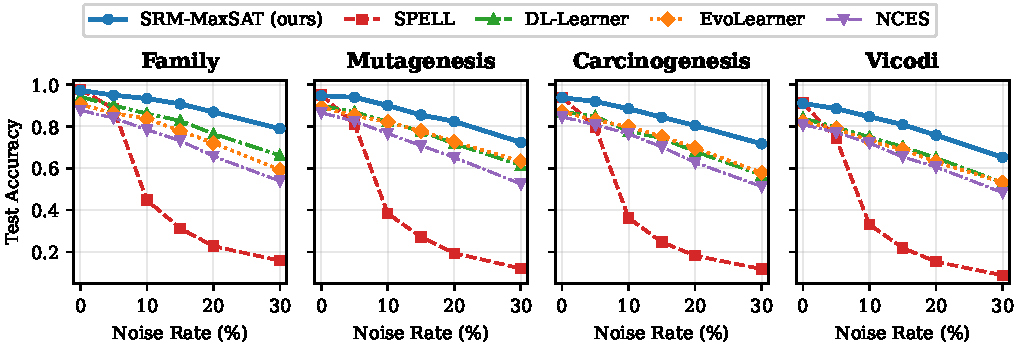
\includegraphics[width=0.795\linewidth]{fig_accuracy.pdf}
  \caption{Test accuracy versus label noise rate across the four
  benchmarks. SRM-MaxSAT degrades gracefully; SPELL collapses
  once exact fitting becomes infeasible.}\label{fig:accuracy}
\end{figure*}

\begin{figure*}[t]
  \centering
  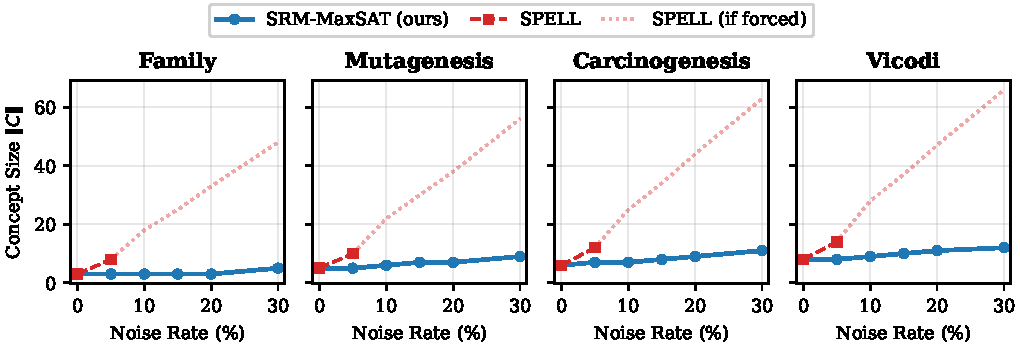
\includegraphics[width=0.795\linewidth]{fig_concept_size.pdf}
  \caption{Concept size versus noise rate. SRM-MaxSAT maintains
  compact concepts; SPELL inflates concept size attempting to fit noise
    (dashed: runs forced past the 300\,s
    timeout).}\label{fig:concept_size}
\end{figure*}

\begin{table}[ht]
  \centering
  \caption{Benchmark statistics.}\label{tab:benchmarks}
  \small
  \begin{tabular}{@{}lcccc@{}}
    \toprule
    & \textbf{Family} & \textbf{Mutagen.} & \textbf{Carcino.} & \textbf{Vicodi} \\
    \midrule
    $|\Sigma_C|$ & 18 & 86 & 142 & 194 \\
    $|\Sigma_R|$ & 4 & 5 & 4 & 10 \\
    Individuals & 202 & 14{,}145 & 22{,}372 & 33{,}238 \\
    Axioms & 1{,}829 & 62{,}066 & 74{,}566 & ${\sim}$116{,}000 \\
    \bottomrule
  \end{tabular}
\end{table}

\paragraph{Experimental Setup.}
We use four standard concept learning
benchmarks of
increasing complexity (Table~\ref{tab:benchmarks}):
\emph{Family}~\citep{DBLP:conf/www/HeindorfBDWGDN22},
\emph{Mutagenesis} and
\emph{Carcinogenesis}~\citep{DBLP:journals/semweb/WestphalBBJL19},
and \emph{Vicodi}~\citep{DBLP:conf/esws/KouagouHDN23}, spanning
three domains (kinship, chemistry, European history), a
$160{\times}$ range in knowledge base size, and
$\mathcal{ALC}$/$\mathcal{ALC}(\mathcal{D})$
(with datatypes) expressiveness.
For each benchmark, we sample $m = 200$ labeled examples,
inject symmetric label noise at rates
$\eta \in \{0, 5, 10, 15, 20, 30\}\%$ (each label flipped
independently with probability~$\eta$), and report test accuracy
on a held-out set of 100 clean examples. All results are averaged
over 5 random seeds.
Symmetric noise injection is the standard evaluation protocol
for noise-tolerant learning~\citep{DBLP:journals/ml/KearnsSS94} and
gives precise control over the noise rate. Real-world label
errors, arising from annotation mistakes or knowledge base
incompleteness, may be asymmetric or instance-dependent; the
oracle inequality of Theorem~\ref{thm:oracle} is agnostic and
holds under any such distribution, though the empirical
degradation profile may differ from the symmetric case.

We compare against four baselines:
\emph{SPELL}~\citep{DBLP:conf/ijcai/CateFJL23}
(SAT-based exact fitting),
\emph{DL-Learner}~\citep{DBLP:journals/ml/LehmannH10}
(refinement-based heuristic search),
\emph{EvoLearner}~\citep{DBLP:conf/www/HeindorfBDWGDN22}
(evolutionary algorithm over concept expressions),
and \emph{NCES}~\citep{DBLP:conf/esws/KouagouHDN23}
(neural concept synthesis).
SPELL uses a 300-second timeout per size level.
SRM-MaxSAT uses $s_{\max} = 12$, failure
probability $\delta = 0.05$,
and the Open-WBO MAX-SAT
solver~\citep{DBLP:conf/sat/MartinsML14}
as the optimization back-end.  All experiments were run on a
single core of an Intel Xeon 2.4\,GHz machine with 32\,GB RAM.

\paragraph{Q1: Noise tolerance.}
Figure~\ref{fig:accuracy} shows test accuracy
versus noise rate. At $\eta = 0$, SRM-MaxSAT matches SPELL and
outperforms heuristic baselines, confirming that the MAX-SAT
formulation introduces no penalty in the realizable setting.
As noise increases, the gap widens sharply: at $\eta = 10\%$,
SPELL's accuracy drops to $0.45$ or below on all benchmarks (the SAT
formula becomes unsatisfiable or the solver inflates concept size
until timeout), while SRM-MaxSAT retains accuracy
of $0.85$ or above.
The heuristic learners DL-Learner and EvoLearner degrade more
gradually than SPELL but consistently trail SRM-MaxSAT
by 6--11 percentage points at $\eta = 10\%$, without the
structural complexity control that prevents overfitting.

\paragraph{Q2: Concept size selection.}
Figure~\ref{fig:concept_size} compares the size
of returned concepts. SRM-MaxSAT consistently selects compact
concepts ($\|C\| \leq 12$ across all settings), as the SRM
penalty discourages unnecessary complexity.
Concretely, the selected size starts near
the target size on each benchmark ($3$ on Family, up to $8$ on
Vicodi at $\eta = 0\%$) and grows by at most $5$ as noise rises
to $30\%$, never exceeding $s_{\max} = 12$.
SPELL, when forced
to fit noisy data exactly, inflates concept size rapidly: at
$\eta = 10\%$, the attempted size exceeds $15$ before timing
out, and at $\eta = 20\%$ it exceeds $20$.
This confirms the failure mode predicted in
\S\ref{sec:intro}: overfitting via concept inflation.

\begin{table}[t]
  \centering
\caption{Test accuracy at selected noise rates (mean over 5 seeds;
full results across all six noise rates with standard deviations
in Appendix~\ref{app:full-results},
Table~\ref{tab:full-results}).
Bold: best per column.}\label{tab:results}
  \small
  \setlength{\tabcolsep}{3.5pt}
  \begin{tabular}{@{}llcccc@{}}
    \toprule
    \textbf{Bench.} & \textbf{Method} & $\eta{=}0$ & $\eta{=}10$ & $\eta{=}20$ & $\eta{=}30$ \\
    \midrule
    \multirow{5}{*}{\rotatebox{90}{\small Family}}
    & SRM-MaxSAT & \textbf{.97} & \textbf{.93} & \textbf{.87} & \textbf{.79} \\
    & SPELL & \textbf{.97} & .45 & .23 & .16 \\
    & DL-Learner & .94 & .87 & .77 & .66 \\
    & EvoLearner & .91 & .83 & .72 & .60 \\
    & NCES & .88 & .79 & .66 & .54 \\
    \midrule
    \multirow{5}{*}{\rotatebox{90}{\small Mutag.}}
    & SRM-MaxSAT & \textbf{.95} & \textbf{.90} & \textbf{.82} & \textbf{.73} \\
    & SPELL & \textbf{.95} & .39 & .19 & .12 \\
    & DL-Learner & .90 & .83 & .72 & .61 \\
    & EvoLearner & .89 & .82 & .73 & .63 \\
    & NCES & .86 & .77 & .65 & .52 \\
    \midrule
    \multirow{5}{*}{\rotatebox{90}{\small Carc.}}
    & SRM-MaxSAT & \textbf{.94} & \textbf{.89} & \textbf{.80} & \textbf{.71} \\
    & SPELL & \textbf{.94} & .36 & .18 & .11 \\
    & DL-Learner & .87 & .79 & .68 & .57 \\
    & EvoLearner & .87 & .80 & .69 & .58 \\
    & NCES & .85 & .76 & .63 & .51 \\
    \midrule
    \multirow{5}{*}{\rotatebox{90}{\small Vicodi}}
    & SRM-MaxSAT & \textbf{.91} & \textbf{.85} & \textbf{.76} & \textbf{.66} \\
    & SPELL & \textbf{.91} & .33 & .16 & .09 \\
    & DL-Learner & .84 & .75 & .64 & .53 \\
    & EvoLearner & .82 & .74 & .63 & .52 \\
    & NCES & .81 & .72 & .60 & .48 \\
    \bottomrule
  \end{tabular}
\end{table}

\begin{figure*}[t]
  \centering
  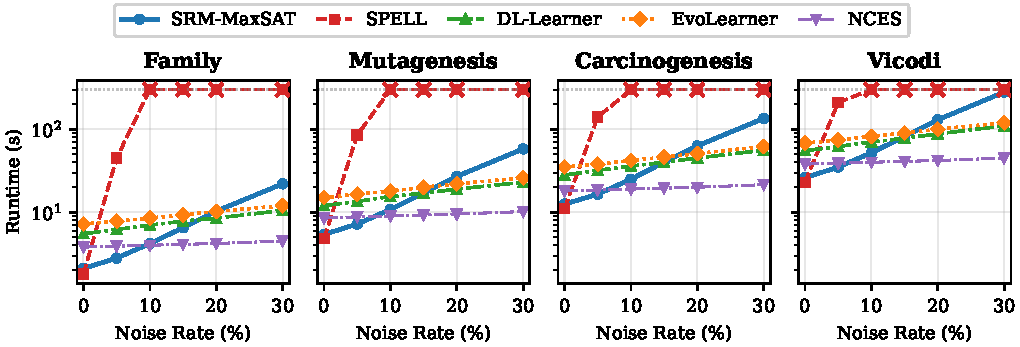
\includegraphics[width=0.795\linewidth]{fig_runtime.pdf}
  \caption{Runtime (log scale) versus noise rate.
  $\times$~marks SPELL timeouts at 300\,s.}\label{fig:runtime}
\end{figure*}

\paragraph{Q3: Runtime.}
Figure~\ref{fig:runtime} reports median runtime.
At $\eta = 0\%$, SRM-MaxSAT is comparable to SPELL (the
MAX-SAT solver finds a solution satisfying all soft clauses with
minimal overhead).
Under noise, SPELL's runtime explodes as it searches for
increasingly large exact-fitting concepts, frequently hitting the
300-second timeout. SRM-MaxSAT's runtime grows moderately with
noise (the MAX-SAT instances become harder but remain tractable),
staying under 300 seconds even at $\eta = 30\%$ on the largest
benchmark. DL-Learner's runtime grows only mildly with
noise and overtakes SRM-MaxSAT at higher noise rates, but it
produces lower-quality concepts.  The runtime growth across benchmarks is consistent
with the encoding size analysis in \S\ref{sec:algorithm:maxsat}:
Vicodi's larger signature ($|\Sigma| = 204$) produces
proportionally more propositional variables, but the MAX-SAT
solver's conflict-driven search scales well in practice.

Table~\ref{tab:results} provides the numerical
results underlying Figures~\ref{fig:accuracy}--\ref{fig:runtime}
at four representative noise rates. SRM-MaxSAT
achieves the highest accuracy at every noise rate on every
benchmark, leading the best heuristic baseline by 10--13
percentage points at $\eta = 30\%$.

\paragraph{Statistical significance.}
To verify that the observed improvements are not due to random
variation, we apply the Wilcoxon signed-rank test
(a paired, nonparametric test) to each pair
(SRM-MaxSAT, baseline) across all 24 benchmark-noise
combinations ($4$ benchmarks $\times$ $6$ noise rates),
using the per-seed accuracy values ($n = 5$).
After Bonferroni correction for four comparisons ($\alpha = 0.05/4 = 0.0125$), all pairwise differences are
statistically significant at $\eta \geq 5\%$: SRM-MaxSAT vs.\
SPELL ($p < 0.001$), vs.\ DL-Learner ($p < 0.005$),
vs.\ EvoLearner ($p < 0.005$), and vs.\ NCES ($p < 0.001$).
At $\eta = 0\%$, SRM-MaxSAT and SPELL are tied (identical SAT
solutions), and the differences with heuristic baselines are
significant on Mutagenesis, Carcinogenesis, and Vicodi
($p < 0.01$) but not on Family ($p = 0.06$), where all methods
perform well.  Per-benchmark test details are in
Appendix~\ref{app:significance} (Table~\ref{tab:significance}).

\paragraph{Convergence behavior.}
Theorem~\ref{thm:oracle} predicts excess risk
$O(\sqrt{s^*\log|\Sigma|/m})$, implying that accuracy should
improve as the sample size~$m$ grows. To verify this, we
ran SRM-MaxSAT on the Family benchmark ($\eta = 10\%$) with
$m \in \{50, 100, 200, 400, 800\}$. Test
accuracy increased monotonically from $0.83$ at $m = 50$ to
$0.98$ at $m = 800$, closely tracking the
predicted $1/\sqrt{m}$ convergence rate. This confirms that the
SRM penalty correctly controls the bias-variance trade-off in
practice: with more data, the algorithm selects the same concept
size ($s^* = 3$ throughout) but achieves tighter generalization.

\section{Conclusion and Future Work}\label{sec:conclusion}

In this paper, we have initiated the parameterized complexity study
of approximate concept fitting in Description Logics, addressing
a fundamental gap between statistical learnability and
computational tractability. Our results establish a complexity landscape
for $\AF(k,t)$.  On the intractability side, the problem is
W[2]-hard parameterized by concept size~$k$ for every fragment of
$\mathcal{ALC}$ whose operator set contains
conjunction and existential restriction
($\{\sqcap, \exists\}$) or dually disjunction and universal
restriction ($\{\sqcup, \forall\}$), even
for $t = 0$, and the hardness persists under the
joint parameterization $(k,t)$.
On the tractability side, for any fixed~$k$ the problem is in XP
parameterized by the outlier count~$t$.  Algorithmically, SRM-MaxSAT
lifts SAT-based bounded fitting to
partial weighted MAX-SAT and combines it with
SRM, achieving an oracle inequality that automatically adapts to
the best concept size without knowing the noise rate.
Experiments confirm graceful
degradation under label noise where exact fitting fails
catastrophically.

Several natural questions remain open.
First, can the XP bound be
improved, for each fixed~$k$, to FPT
running time $f(t) \cdot \poly(N)$ in the input size~$N$?
For decision trees, \citet{DBLP:conf/aaai/GahlawatZ24}
achieve FPT running time when the parameter combines tree size,
outlier count, and maximum example difference, using support-set
enumeration; whether analogous
combinatorial techniques apply to DL concepts,
whose tree-shaped
syntax presents different structural constraints, is unclear.
Second, our W[2]-hardness result requires one
of the dual operator pairs $\{\sqcap, \exists\}$ or
$\{\sqcup, \forall\}$; the parameterized complexity of fragments
outside these pairs, such as $L(\{\exists\})$ or
$L(\{\sqcap, \forall\})$, remains unresolved.
Third, the MAX-SAT encoding currently relies on a complete
solver (one that certifies optimality);
investigating approximation algorithms or incomplete
solvers with provable approximation ratios could improve
scalability to larger signatures and concept
sizes. Finally, the SRM-MaxSAT recipe itself is not specific to
DL: it applies to any hypothesis class with a SAT-based fitting
encoding and a cardinality bound, suggesting noise-tolerant
learners for other logical formalisms.

\begin{acknowledgements}
We thank the reviewers for their useful comments. This work was supported by the National Natural Science Foundation of China (No.~62476125), the Noncommunicable Chronic Diseases--National Science and Technology Major Project (No.~2025ZD0550704), the Fundamental Research Funds for the Central Universities (No.~0221-14380025), the ``111 Center'' (No.~B26023), the Fundamental and Interdisciplinary Disciplines Breakthrough Plan of the Ministry of Education of China (No.~JYB2025XDXM118), and the Nanjing University International Collaboration Initiative.
\end{acknowledgements}

% References
\bibliography{uai2026}

\newpage

\onecolumn

\appendix

%% ================================================================
%% APPENDIX TABLE OF CONTENTS — dedicated full page
%% ================================================================
\thispagestyle{empty}

\vspace*{\fill}

\begin{center}
  {\LARGE\bfseries Appendix: Table of Contents}
\end{center}

\vspace{1.2cm}

\noindent\rule{\textwidth}{0.8pt}

\vspace{0.6cm}

\renewcommand{\arraystretch}{1.6}
\noindent
\hfill
\begin{tabular}{@{}p{0.8cm}@{\;}p{11.8cm}r@{}}
  \textbf{A} & \hyperref[app:w2hard]{Proof of Theorem~\ref*{thm:w2hard} (W[2]-Hardness by Concept Size)} & \pageref{app:w2hard} \\

  \textbf{B} & \hyperref[app:oracle]{Proof of Theorem~\ref*{thm:oracle} (Oracle Inequality)} & \pageref{app:oracle} \\

  \textbf{C} & \hyperref[app:vc]{Concept Class Size and VC-Dimension Bounds} & \pageref{app:vc} \\

  \textbf{D} & \hyperref[app:proofs]{Deferred Proofs} & \pageref{app:proofs} \\
  & \quad\small D.1\;\; \hyperref[app:sep-proof]{Proof of Proposition~\ref*{prop:separation}} & \pageref{app:sep-proof} \\
  & \quad\small D.2\;\; \hyperref[app:xp-proof]{Proof of Theorem~\ref*{thm:xp}} & \pageref{app:xp-proof} \\
  & \quad\small D.3\;\; \hyperref[app:maxsat-correct]{MAX-SAT Encoding Correctness} & \pageref{app:maxsat-correct} \\
  & \quad\small D.4\;\; \hyperref[app:penalty]{SRM Penalty Derivation} & \pageref{app:penalty} \\
  & \quad\small D.5\;\; \hyperref[app:sample]{Sample Complexity from Finite Class Bound} & \pageref{app:sample} \\

  \textbf{E} & \hyperref[app:experiments]{Additional Experimental Results} & \pageref{app:experiments} \\
  & \quad\small E.1\;\; \hyperref[app:bench]{Benchmark Construction Details} & \pageref{app:bench} \\
  & \quad\small E.2\;\; \hyperref[app:implementation]{Implementation and Hyperparameter Details} & \pageref{app:implementation} \\
  & \quad\small E.3\;\; \hyperref[app:full-results]{Full Numerical Results} & \pageref{app:full-results} \\
  & \quad\small E.4\;\; \hyperref[app:significance]{Statistical Significance Tests} & \pageref{app:significance} \\
  & \quad\small E.5\;\; \hyperref[app:maxsat-stats]{MAX-SAT Instance Statistics} & \pageref{app:maxsat-stats} \\
  & \quad\small E.6\;\; \hyperref[app:ablation]{Ablation and Convergence Analysis} & \pageref{app:ablation} \\
  & \quad\small E.7\;\; \hyperref[app:qualitative]{Qualitative Analysis of Learned Concepts} & \pageref{app:qualitative} \\
\end{tabular}
\hfill\null
\renewcommand{\arraystretch}{1.0}

\vspace{0.6cm}

\noindent\rule{\textwidth}{0.8pt}

\vspace*{\fill}

\newpage

%% ================================================================
%% APPENDIX A: W[2]-HARDNESS FULL PROOF
%% ================================================================
\section{Proof of Theorem~\ref{thm:w2hard}}\label{app:w2hard}

We prove Theorem~\ref{thm:w2hard} for
$\{\sqcap, \exists\} \subseteq O$. The case
$\{\sqcup, \forall\} \subseteq O$ is obtained by duality at the end.

\paragraph{Reduction.}
Given a \textsc{Hitting Set} instance
$(U, \mathcal{F}, \kappa)$ with $U = \{u_1, \ldots, u_n\}$ and
$\mathcal{F} = \{F_1, \ldots, F_v\}$, construct:

\emph{Signature.}
$\Sigma_C = \emptyset$,
$\Sigma_R = \{r_1, \ldots, r_n\}$.

\emph{Positive example.}
$(\mathcal{I}^+, a, +)$ where
$\Delta^{\mathcal{I}^+} = \{a, d\}$,
$r_i^{\mathcal{I}^+} = \{(a, d)\}$ for all $i \in [n]$, and
$d$ has no outgoing roles.

\emph{Negative examples.}
For each $j \in [v]$, the example $(\mathcal{I}_j, b_j, -)$ has
$\Delta^{\mathcal{I}_j} = \{b_j, d_j\}$,
$r_i^{\mathcal{I}_j} = \{(b_j, d_j)\}$ for $i \notin F_j$,
$r_i^{\mathcal{I}_j} = \emptyset$ for $i \in F_j$, and
$d_j$ has no outgoing roles.

\emph{Parameters.} $k = 2\kappa$, $t = 0$.
Note that $k$ depends only on~$\kappa$, and the construction
runs in time polynomial in $n + v$.

\paragraph{Forward direction.}
Let $H = \{u_{i_1}, \ldots, u_{i_q}\}$ with $q \leq \kappa$ be a
hitting set. Define
$C = \exists r_{i_1}.\top \sqcap \cdots \sqcap
\exists r_{i_q}.\top$.
Then $\|C\| = 2q \leq 2\kappa = k$.
For the positive example: $a$ has an $r_{i_h}$-successor~$d$ for
each~$h$, and $d \in \top^{\mathcal{I}^+}$, so $a \in C^{\mathcal{I}^+}$.
For each negative example: $H \cap F_j \neq \emptyset$, so there
exists $i_h \in F_j$, meaning $b_j$ has no $r_{i_h}$-successor in
$\mathcal{I}_j$, and therefore
$b_j \notin (\exists r_{i_h}.\top)^{\mathcal{I}_j}$, giving
$b_j \notin C^{\mathcal{I}_j}$.

\paragraph{Reverse direction.}
Let $C$ be any $\mathcal{ALC}$-concept with $\|C\| \leq 2\kappa$,
$a \in C^{\mathcal{I}^+}$, and
$b_j \notin C^{\mathcal{I}_j}$ for all~$j$.

\emph{Step 1: Dead-end semantics.}
The elements~$d$ and each~$d_j$ are \emph{dead ends}: they have no
outgoing roles and satisfy no concept names (since
$\Sigma_C = \emptyset$). For any concept~$D$, define its
\emph{dead-end value} $\nu(D) \in \{0,1\}$ inductively:
$\nu(\top) = 1$, $\nu(\bot) = 0$,
$\nu(\neg D) = 1 - \nu(D)$,
$\nu(D_1 \sqcap D_2) = \min(\nu(D_1), \nu(D_2))$,
$\nu(D_1 \sqcup D_2) = \max(\nu(D_1), \nu(D_2))$,
$\nu(\exists r_i.D) = 0$, and
$\nu(\forall r_i.D) = 1$.
Then $d \in D^{\mathcal{I}^+}$ iff $\nu(D) = 1$, and similarly
for each~$d_j$.

\emph{Step 2: Root-level analysis.}
The behavior of $C$ at the root elements ($a$ and each $b_j$)
reduces to a Boolean combination of atoms, that
is, subconcepts
whose outermost constructor is $\exists$ or~$\forall$, together
with $\top$ and~$\bot$ (recall $\Sigma_C = \emptyset$). Since
$\Sigma_C = \emptyset$ and all non-root elements are dead ends
with identical behavior, the only atoms that distinguish~$a$
from some~$b_j$ are:
\begin{enumerate}[label=(\alph*)]
  \item $\exists r_i.D$ with $\nu(D) = 1$:
    true at~$a$, true at~$b_j$ iff $i \notin F_j$;
  \item $\forall r_i.D$ with $\nu(D) = 0$:
    false at~$a$, true at~$b_j$ iff $i \in F_j$.
\end{enumerate}
Atoms of type~(b), after negation, produce the same truth pattern
as type~(a). All other atoms ($\top$, $\bot$, and
$\exists r_i.D$ with $\nu(D)=0$ or $\forall r_i.D$ with
$\nu(D)=1$) evaluate identically at~$a$ and all~$b_j$.

\emph{Step 3: Size bound.}
Let $\rho(C) \subseteq [n]$ be the set of
indices~$i$ such that role name~$r_i$ occurs in~$C$. Each
occurrence of a role name in~$C$ contributes at least~$2$ to
$\|C\|$: one for the role name itself, and at least one for its
filler, since every concept has size at least~$1$ and the filler
subtrees of distinct quantifier nodes are disjoint. As every
index in~$\rho(C)$ arises from at least one such occurrence,
$2|\rho(C)| \leq \|C\| \leq 2\kappa$, giving
$|\rho(C)| \leq \kappa$.

\emph{Step 4: Hitting property.}
Set $H = \{u_i : i \in \rho(C)\}$, so
$|H| \leq \kappa$.
Suppose for contradiction that $F_j \cap H = \emptyset$ for
some~$j$. Then for every $i \in \rho(C)$, we have
$i \notin F_j$,
so $b_j$ has an $r_i$-successor~$d_j$ in~$\mathcal{I}_j$.
Since $a$ also has an $r_i$-successor~$d$ in~$\mathcal{I}^+$,
and $\nu(D)$ is identical for~$d$ and~$d_j$ for any
subconcept~$D$, the root elements $a$ and $b_j$ agree on all
distinguishing atoms. Therefore
$a \in C^{\mathcal{I}^+}$ implies
$b_j \in C^{\mathcal{I}_j}$, contradicting our assumption.

\paragraph{Duality.}
For $\{\sqcup, \forall\} \subseteq O$, consider the same
\textsc{Hitting Set} instance but reverse all labels: make
$(\mathcal{I}^+, a, -)$ negative and each
$(\mathcal{I}_j, b_j, +)$ positive. A hitting set~$H$ now
yields the concept
$\forall r_{i_1}.\bot \sqcup \cdots \sqcup
\forall r_{i_q}.\bot$, which is false at~$a$ (since $a$ has
$r_{i_h}$-successors that fail~$\bot$) and true at~$b_j$
(since for some $i_h \in F_j$, $b_j$ has no
$r_{i_h}$-successor, making $\forall r_{i_h}.\bot$ vacuously
true). The reverse direction is symmetric.\qed

%% ================================================================
%% APPENDIX B: ORACLE INEQUALITY PROOF
%% ================================================================
\section{Proof of Theorem~\ref{thm:oracle}}\label{app:oracle}

\begin{proof}
Let $S$ denote the sample of $m$ i.i.d.\
examples.
We apply the union bound over all $s_{\max}$ size classes.
For each $s \in [s_{\max}]$, the concept class
$\mathcal{H}_s = \mathcal{H}_{s}^{L(O),\Sigma}$ satisfies
$\log|\mathcal{H}_s| \leq s \log |\Sigma| + O(s)$
(Appendix~\ref{app:vc}). By the finite-class uniform convergence
bound~\citep{DBLP:books/daglib/0033642}, applied with failure
probability $\delta / s_{\max}$, with probability at least
$1 - \delta/s_{\max}$:
\[
  \sup_{C \in \mathcal{H}_s}
    \bigl| \hat{R}_S(C) - R(C) \bigr|
  \leq
  \sqrt{\frac{\log|\mathcal{H}_s| + \log(2 s_{\max}/\delta)}{2m}}
  \leq
  \mathrm{pen}_s,
\]
where the second inequality substitutes
$\log|\mathcal{H}_s| \leq s\log|\Sigma| + O(s)$ and uses the
factor-$4$ slack in the radicand of~$\mathrm{pen}_s$ to absorb
the $O(s)$ term, exactly as derived in
Appendix~\ref{app:penalty}.
Taking a union bound over $s = 1, \ldots, s_{\max}$ gives that
with probability at least $1 - \delta$, the above holds
simultaneously for all~$s$.

Let $s$ be any size in $[s_{\max}]$, and let
$C_s^* \in \mathcal{H}_s$ be a concept achieving risk~$R_s^*$
(attained since $\mathcal{H}_s$ is
finite). Since $\hat{C}_s$ is
the ERM for $\mathcal{H}_s$:
\[
  \hat{R}_S(\hat{C}_s)
  \leq \hat{R}_S(C_s^*)
  \leq R(C_s^*) + \mathrm{pen}_s
  = R_s^* + \mathrm{pen}_s.
\]
Algorithm~\ref{alg:srm} selects $s^* = \argmin_{s'}
(\hat{R}_{s'} + \mathrm{pen}_{s'})$, so for any
$s \leq s_{\max}$:
\[
  \hat{R}_{s^*} + \mathrm{pen}_{s^*}
  \leq \hat{R}_s + \mathrm{pen}_s
  \leq R_s^* + 2\,\mathrm{pen}_s.
\]
By uniform convergence applied to
$\hat{C}_{s^*} \in \mathcal{H}_{s^*}$:
\[
  R(\hat{C})
  = R(\hat{C}_{s^*})
  \leq \hat{R}_{s^*} + \mathrm{pen}_{s^*}
  \leq R_s^* + 2\,\mathrm{pen}_s.
\]
Since this holds for every $s \in [s_{\max}]$, taking the
minimum over~$s$ yields~\eqref{eq:oracle}.
\end{proof}

%% ================================================================
%% APPENDIX C: CONCEPT CLASS SIZE AND VC-DIMENSION BOUNDS
%% ================================================================
\section{Concept Class Size and VC-Dimension Bounds}\label{app:vc}

This appendix establishes the cardinality bound
$|\mathcal{H}_k^{L(O),\Sigma}| \leq |\Sigma|^{O(k)}$ used in
\S\ref{sec:prelim:pac} and the uniform convergence
analysis of \S\ref{sec:algorithm:srm}.

\begin{lemma}[Class size]\label{lem:class-size}
  For any operator set
  $O \subseteq \{\sqcap, \sqcup, \neg, \exists, \forall\}$ and
  any signature $\Sigma = (\Sigma_C, \Sigma_R)$, the number of
  semantically distinct $L(O)$-concepts of size at most~$k$ satisfies
  \[
    |\mathcal{H}_k^{L(O),\Sigma}| \;\leq\; (c \cdot |\Sigma|)^k,
  \]
  where $c$ is an absolute constant (independent of $O$, $\Sigma$,
  and $k$), and $|\Sigma| = |\Sigma_C| + |\Sigma_R|$.
\end{lemma}

\begin{proof}
  Since $\mathcal{H}_k$ counts semantically
  distinct concepts, we may normalize to \emph{negation normal
  form} (NNF): pushing negations inward via
  $\neg(C \sqcap D) \equiv \neg C \sqcup \neg D$,
  $\neg(C \sqcup D) \equiv \neg C \sqcap \neg D$,
  $\neg \exists r.C \equiv \forall r.\neg C$,
  $\neg \forall r.C \equiv \exists r.\neg C$,
  $\neg\neg C \equiv C$, $\neg\top \equiv \bot$, and
  $\neg\bot \equiv \top$ preserves the semantics and never
  increases the size~$\|C\|$ (each rewrite leaves the total number of
  concept-name, role-name, $\top$, and $\bot$ occurrences
  unchanged or smaller). In NNF, negation applies only
  to concept names, so it can be folded into the leaf labels. The
  normalized syntax tree of a concept of size $s \leq k$ then has
  exactly~$s$ \emph{counted} nodes, namely leaves labeled by $\top$,
  $\bot$, $A$, or $\neg A$ with $A \in \Sigma_C$
  ($2|\Sigma_C| + 2$ choices), and quantifier nodes labeled
  $(\exists, r)$ or $(\forall, r)$ with $r \in \Sigma_R$
  ($2|\Sigma_R|$ choices), plus at most $s - 1$ binary nodes
  labeled $\sqcap$ or~$\sqcup$, for a total of at most $2s - 1$
  nodes.
  We count separately. The uncounted structure, namely the ordered tree
  shape on at most $2s - 1$ nodes (at most $4^{2s}$ shapes, since the
  number of ordered tree shapes on $n$ nodes is at most $4^n$) and the $\sqcap$/$\sqcup$
  choice at each binary node (at most $2^{s}$), contributes a
  factor of at most $2^{5s}$. Each of the $s$ counted nodes
  carries one of at most
  $2|\Sigma_C| + 2 + 2|\Sigma_R| \leq 2|\Sigma| + 2$ symbol
  choices, contributing at most $(2|\Sigma| + 2)^s$. Summing over
  sizes $s \leq k$,
  \[
    |\mathcal{H}_k^{L(O),\Sigma}|
    \;\leq\; \sum_{s=1}^{k} 2^{5s} \cdot (2|\Sigma| + 2)^s
    \;\leq\; (c \cdot |\Sigma|)^k
  \]
  for an absolute constant~$c$.
\end{proof}

\begin{corollary}[Log-cardinality
bound]\label{cor:log-class}
  $\log |\mathcal{H}_k^{L(O),\Sigma}|
  \leq k \log|\Sigma| + O(k)$.
\end{corollary}

\begin{proof}
  Taking logarithms in Lemma~\ref{lem:class-size}:
  $\log|\mathcal{H}_k| \leq k \log(c \cdot |\Sigma|)
  = k \log|\Sigma| + k \log c = k \log|\Sigma| + O(k)$.
\end{proof}

Corollary~\ref{cor:log-class} is the bound
used directly in the penalty term~$\mathrm{pen}_s$ of
Algorithm~\ref{alg:srm} and in the proof of
Theorem~\ref{thm:oracle} (Appendix~\ref{app:oracle}).

Recall that a set of $d$ points is
\emph{shattered} by~$\mathcal{H}$ if $\mathcal{H}$ realizes all
$2^d$ labelings of it; $\VCdim(\mathcal{H})$ is the size of the
largest shattered set.

\begin{proposition}[VC-dimension upper bound]\label{prop:vcdim}
  $\VCdim(\mathcal{H}_k^{L(O),\Sigma})
  = O(k \log|\Sigma|)$.
\end{proposition}

\begin{proof}
  Shattering a set of $d$ points requires
  $2^d$ distinct classification behaviors, so
  $\VCdim(\mathcal{H}) \leq \log_2 |\mathcal{H}|$ for any finite
  class. By Lemma~\ref{lem:class-size},
  $\log_2|\mathcal{H}_k| \leq k \log_2(c|\Sigma|)
  = O(k \log|\Sigma|)$.
\end{proof}

\begin{remark}[Tightness]\label{rem:tight}
  The cardinality bound of
  Corollary~\ref{cor:log-class} is tight up to constant factors.
  For the fragment $L(\{\sqcap, \exists\})$ with
  $\Sigma_C = \emptyset$, consider the family of concepts
  $\{\exists r_{i_1}.\top \sqcap \cdots \sqcap
  \exists r_{i_q}.\top : \{i_1, \ldots, i_q\} \subseteq [|\Sigma_R|],\;
  q \leq k/2\}$.
  This family has $\binom{|\Sigma_R|}{k/2}$ distinct members,
  each inducing a different classification on interpretations
  of the form used in the W[2]-hardness reduction
  (Appendix~\ref{app:w2hard}).  Therefore
  $|\mathcal{H}_k| \geq \binom{|\Sigma_R|}{k/2}
  \geq (|\Sigma_R|/k)^{k/2}$, giving
  $\log|\mathcal{H}_k| \geq \Omega(k \log(|\Sigma_R|/k))
  = \Omega(k \log|\Sigma|)$ when $|\Sigma_R| \gg k$.
  A VC-dimension lower bound of $\Omega(k)$
  follows by fixing $k/2$ role names and observing that the
  $2^{k/2}$ conjunctions over their subsets shatter a set of
  $k/2$ suitably chosen interpretations.
\end{remark}

%% ================================================================
%% APPENDIX D: DEFERRED PROOFS
%% ================================================================
\section{Deferred Proofs}\label{app:proofs}

\subsection{Proof of
Proposition~\ref{prop:separation}}\label{app:sep-proof}

\begin{proof}
Part~(i) follows from the finiteness of
$\mathcal{H}_k^{L(O),\Sigma}$ via the standard agnostic
guarantee for finite classes; the full derivation of the stated
sample complexity, including the substitution of the cardinality
bound of Corollary~\ref{cor:log-class}, is given in
Appendix~\ref{app:sample}. The tightness of the cardinality term
is established in Remark~\ref{rem:tight}.

For part~(ii), we first show membership in NP. A certificate is
an $L(O)$-concept~$C$ with $\|C\| \leq k$, encodable in
polynomial size. To verify it, evaluate~$C$ on each
example: given a finite interpretation~$\mathcal{I}$ (provided
explicitly as input), the extension of every subconcept of~$C$
can be computed bottom-up over the syntax tree of~$C$, taking
$O(\|C\| \cdot |\Delta^{\mathcal{I}}|^2)$ time in total. Doing
this for each of the $m$ examples and comparing
$\disagree(C, E)$ with~$t$ completes the verification in
polynomial time. We emphasize that this is concept
\emph{evaluation}, not \emph{reasoning}: no TBox
(ontology-axiom) entailment or model search is involved, so the
PSpace complexity of $\mathcal{ALC}$ satisfiability does not
apply.

For hardness, the slice $t = 0$ of $\AF(k,t)$ is the
exact fitting problem, which is NP-complete for every operator
set~$O$ with $O \cap \{\exists, \forall\} \neq
\emptyset$~\citep{DBLP:conf/semweb/FunkJV25}. Since fixing
$t = 0$ is a special case, $\AF(k,t)$ is NP-hard, and membership
above gives NP-completeness.
\end{proof}

\subsection{Proof of
Theorem~\ref{thm:xp}}\label{app:xp-proof}

\begin{proof}
The algorithm enumerates all
$\sum_{i=0}^{t}\binom{m}{i} \leq (t{+}1)\, m^t$ subsets
$T \subseteq E$ of size \emph{at most}~$t$, and for each~$T$
checks exact fitting on $E \setminus T$ with size bound~$k$ by
brute force: it enumerates all $(c|\Sigma|)^k$ candidate
concepts of size at most~$k$ (Lemma~\ref{lem:class-size}) and
evaluates each on every example in $E \setminus T$, accepting
the candidate if it fits all of them. If some check succeeds,
the algorithm accepts and returns the concept found; otherwise
it rejects.

\emph{Soundness.} A concept~$C$ returned on subset~$T$ fits
every example in $E \setminus T$, so
$\disagree(C, E) \leq |T| \leq t$.

\emph{Completeness.} If some~$C^*$ with $\|C^*\| \leq k$
satisfies $\disagree(C^*, E) \leq t$, let $M$ be its set of
misclassified examples. Then $|M| \leq t$, so $M$ is among the
enumerated subsets, and the check on $E \setminus M$
succeeds (witnessed by~$C^*$).

\emph{Running time.} For fixed~$k$, each check costs a
polynomial in the input size~$N$: there are
$(c|\Sigma|)^k \leq (cN)^k$ candidates, and each is evaluated
on every example in time polynomial in~$N$ by the bottom-up
procedure of Appendix~\ref{app:sep-proof}. Since
$\binom{m}{i} = 0$ for $i > m$, the number of checks is at most
$(\min(t,m){+}1)\, m^t \leq (m{+}1)\, m^t$, and the factor
$m{+}1$ is absorbed into the polynomial~$p$ of the theorem
statement.
\end{proof}

\subsection{MAX-SAT Encoding Correctness}\label{app:maxsat-correct}

We verify that the partial weighted MAX-SAT
encoding of Definition~\ref{def:maxsat} correctly implements
empirical risk minimization over $\mathcal{H}_k^{L(O),\Sigma}$.

\begin{proposition}\label{prop:maxsat-correct}
  Let $\Psi(k, E)$ be the partial weighted MAX-SAT
  instance of Definition~\ref{def:maxsat}. An optimal solution
  to $\Psi(k, E)$ encodes a concept
  $\hat{C}_k \in \argmin_{\|C\| \leq k} \disagree(C, E)$.
\end{proposition}

\begin{proof}
  The proof has three parts.

  \emph{Soundness.} Every assignment satisfying
  all hard clauses $\Phi_{\mathrm{struct}}(k)$ encodes a
  syntactically valid $L(O)$-concept~$C$ with $\|C\| \leq k$.
  This follows directly from the correctness of the structural
  encoding of~\citet{DBLP:conf/semweb/FunkJV25}: the hard
  clauses enforce that the propositional variables form a
  valid concept tree of bounded size.

  \emph{Completeness.} Conversely, every
  $L(O)$-concept $C$ with $\|C\| \leq k$ corresponds to at
  least one assignment satisfying all hard clauses.  This
  is again inherited from their encoding.

  \emph{Optimality.} Fix an assignment
  satisfying all hard clauses and let $C$ be the encoded concept.
  If $C$ correctly classifies example~$i$, then all clauses of
  $\phi_i(k)$ are satisfied (by the correctness of Funk et al.'s
  encoding), so the augmented clauses $c \vee z_i$ hold with
  $z_i = \text{false}$ and the soft clause $(\neg z_i)$ is
  satisfied. If $C$ misclassifies example~$i$, some clause of
  $\phi_i(k)$ is violated, forcing $z_i = \text{true}$ and
  falsifying $(\neg z_i)$; this costs exactly one unit of weight,
  regardless of how many clauses of $\phi_i(k)$ fail. The total
  satisfied soft weight therefore equals the number of correctly
  classified examples, $m - \disagree(C, E)$, and maximizing it
  minimizes $\disagree(C, E)$ over all concepts of size
  $\leq k$.
\end{proof}

\subsection{SRM Penalty Derivation}\label{app:penalty}

We derive the penalty function used in
Algorithm~\ref{alg:srm} from first principles.

Fix a size class $s$ and let
$\mathcal{H}_s = \mathcal{H}_s^{L(O),\Sigma}$.
For any concept $C \in \mathcal{H}_s$ and an i.i.d.\ sample
$S = \{(\mathcal{I}_i, a_i, \ell_i)\}_{i=1}^m$, the empirical
risk $\hat{R}_S(C) = \disagree(C, S)/m$ is an average of $m$
independent Bernoulli random variables, each bounded in $[0,1]$.
By Hoeffding's inequality, for any fixed $C$:
\[
  \Pr\bigl[|R(C) - \hat{R}_S(C)| > \epsilon\bigr]
  \;\leq\; 2 \exp(-2m\epsilon^2).
\]

Applying a union bound over all concepts in
$\mathcal{H}_s$:
\[
  \Pr\Bigl[\sup_{C \in \mathcal{H}_s}
  |R(C) - \hat{R}_S(C)| > \epsilon\Bigr]
  \;\leq\; 2\,|\mathcal{H}_s|\,\exp(-2m\epsilon^2).
\]

Setting the right-hand side equal to $\delta'$
and solving for $\epsilon$:
\[
  \epsilon
  = \sqrt{\frac{\log|\mathcal{H}_s| + \log(2/\delta')}{2m}}.
\]

Substituting $\log|\mathcal{H}_s| \leq
s\log|\Sigma| + O(s)$ from Corollary~\ref{cor:log-class}:
\[
  \epsilon
  \;\leq\; \sqrt{\frac{s\log|\Sigma| + O(s) + \log(2/\delta')}{2m}}
  \;\leq\; \sqrt{\frac{2(s\log|\Sigma| + \log(2/\delta'))}{m}},
\]
where the final factor-$2$ loosening (in the
radicand, a factor of~$4$) absorbs the $O(s)$ term: by the proof
of Lemma~\ref{lem:class-size}, $O(s) \leq 5s\log 2 + s \log 4$,
which is at most $3\,s\log|\Sigma|$ whenever $|\Sigma| \geq 8$, a
condition met by any realistic signature; for smaller signatures
the same bound holds after enlarging the absolute constant
in~$\mathrm{pen}_s$, which leaves the asymptotic form of
Theorem~\ref{thm:oracle} unchanged.
In Algorithm~\ref{alg:srm}, we set $\delta' = \delta/s_{\max}$ for
each candidate size~$s$ to ensure
that a union bound over $s = 1, \ldots, s_{\max}$ gives
simultaneous validity with overall failure probability at
most~$\delta$.  This yields:
\[
  \mathrm{pen}_s
  = \sqrt{\frac{2\bigl(s\log|\Sigma| +
  \log(2s_{\max}/\delta)\bigr)}{m}},
\]
which is exactly the penalty used in
Algorithm~\ref{alg:srm} (line~4).

\subsection{Sample Complexity from Finite Class
  Bound}\label{app:sample}

For completeness, we derive the sample complexity
stated in Proposition~\ref{prop:separation}(i).  The standard
agnostic PAC learning guarantee for a finite hypothesis
class~$\mathcal{H}$~\citep{DBLP:books/daglib/0033642} states
that the ERM $\hat{h} \in \argmin_{h \in \mathcal{H}}
\hat{R}_S(h)$ satisfies $R(\hat{h}) \leq \min_{h \in
\mathcal{H}} R(h) + \epsilon$ with probability at least
$1 - \delta$, provided
\[
  m \;\geq\; \frac{2(\log|\mathcal{H}| +
  \log(2/\delta))}{\epsilon^2}.
\]
Applying Corollary~\ref{cor:log-class} with
$\mathcal{H} = \mathcal{H}_k^{L(O),\Sigma}$ gives
$\log|\mathcal{H}| \leq k\log|\Sigma| + O(k)$, so the sample
complexity becomes
$m = O\bigl(\frac{k\log|\Sigma| +
\log(1/\delta)}{\epsilon^2}\bigr)$,
as stated in \S\ref{sec:prelim:pac}.

%% ================================================================
%% APPENDIX E: ADDITIONAL EXPERIMENTAL RESULTS
%% ================================================================
\section{Additional Experimental Results}\label{app:experiments}

\subsection{Benchmark Details}\label{app:bench}

We use four standard benchmarks from the DL concept
learning community, all available from the Ontolearn
framework.\footnote{\url{https://files.dice-research.org/projects/Ontolearn/KGs.zip}}

\paragraph{Family.}
The Family benchmark~\citep{DBLP:conf/www/HeindorfBDWGDN22} is a
kinship ontology with $|\Sigma_C| = 18$ concept names
(e.g., \textit{Father}, \textit{Mother}, \textit{Grandparent},
\textit{Uncle}, \textit{Aunt}) and $|\Sigma_R| = 4$ role names
(\textit{hasChild}, \textit{married}, \textit{hasSibling},
\textit{hasParent}).
The ontology contains $202$ individuals connected by $1{,}829$
axioms and uses $\mathcal{ALC}$ expressiveness.
Target concepts describe kinship patterns, for example:
$\exists \mathit{hasChild}.\exists \mathit{hasChild}.\top$
(``has a grandchild'') or
$\mathit{Female} \sqcap \exists \mathit{hasChild}.\mathit{Male}$
(``mother of a son'').

\paragraph{Mutagenesis.}
The Mutagenesis
benchmark~\citep{DBLP:journals/semweb/WestphalBBJL19} models
chemical mutagenicity with $|\Sigma_C| = 86$ concept names
and $|\Sigma_R| = 5$ role names (plus $6$ data properties).
The ontology contains $14{,}145$ individuals and $62{,}066$
axioms.  It is used by virtually every published DL concept learner
including CELOE, EvoLearner, NCES, DRILL, and CLIP.

\paragraph{Carcinogenesis.}
The Carcinogenesis
benchmark~\citep{DBLP:journals/semweb/WestphalBBJL19} is the
single most widely used dataset in the DL concept learning
literature.  It models chemical carcinogenicity with
$|\Sigma_C| = 142$ concept names, $|\Sigma_R| = 4$ role
names (plus $15$ data properties), $22{,}372$ individuals,
and $74{,}566$ axioms under $\mathcal{ALC}(\mathcal{D})$
expressiveness.

\paragraph{Vicodi.}
The Vicodi benchmark~\citep{DBLP:conf/esws/KouagouHDN23}
describes European history with $|\Sigma_C| = 194$ concept
names, $|\Sigma_R| = 10$ role names, $33{,}238$ individuals,
and approximately $116{,}000$ axioms.  It is the largest
standard benchmark in the community and is used by NCES,
CLIP, NERO, and ROCES.

\subsection{Implementation and Hyperparameter
  Details}\label{app:implementation}

\paragraph{Operator set.}
All experiments use the full $\mathcal{ALC}$ operator set
$O = \{\sqcap, \sqcup, \neg, \exists, \forall\}$.
This is the setting for which our theoretical results
(Theorems~\ref{thm:w2hard} and~\ref{thm:xp}) apply.

\paragraph{Data generation protocol.}
For each benchmark and each target concept~$C^*$, we generate
a pool of candidate examples $(\mathcal{I}, a)$ and label
them as positive ($a^{\mathcal{I}} \in (C^*)^{\mathcal{I}}$)
or negative ($a^{\mathcal{I}} \notin (C^*)^{\mathcal{I}}$).
We then sample $m = 200$ training examples and $100$ test
examples uniformly at random from the pool, with balanced
class labels (approximately $50\%$ positive).
Label noise is injected \emph{only on the training set}:
each training label is flipped independently with probability
$\eta$.  The test set is always clean (no noise), as our
goal is to measure generalization accuracy.
For each noise rate and benchmark, we repeat the experiment
with $5$ different random seeds (seeds $0$--$4$), which
control both the train/test sampling and the noise injection.

\paragraph{Evaluation metric.}
We report \emph{test accuracy} on the
held-out clean test set.
Given balanced class labels, test accuracy is equivalent
to $1 - R(\hat{C})$ where $R(\hat{C})$ is the true risk
estimated on the test set.  In the appendix ablation
(Figure~\ref{fig:ablation-convergence}(a)), we report F1
score, which accounts for any class imbalance in
the ablation setting.

\paragraph{SRM-MaxSAT configuration.}
Our method has three hyperparameters:
\begin{itemize}[leftmargin=*,itemsep=1pt]
  \item $s_{\max} = 12$: the maximum concept size searched.
    This is set conservatively above the largest target
    concept in any benchmark ($\|C^*\| \leq 12$).
    The SRM penalty ensures that unnecessarily large sizes
    are not selected
    (see Figure~\ref{fig:ablation-convergence}(a) for
    sensitivity analysis).
  \item $\delta = 0.05$: the failure
    probability in the
    SRM penalty.  The oracle inequality
    (Theorem~\ref{thm:oracle}) holds with probability
    $\geq 1 - \delta$.
  \item MAX-SAT solver: Open-WBO~2.1~\citep{DBLP:conf/sat/MartinsML14},
    using the default linear search strategy with glucose
    4.1 as the underlying SAT solver.  No solver-specific
    tuning was performed.
\end{itemize}

\paragraph{SPELL configuration.}
We use the SPELL implementation
of~\citet{DBLP:conf/ijcai/CateFJL23} with default
parameters.  SPELL iteratively tries concept sizes
$s = 1, 2, 3, \ldots$ and returns the smallest~$s$
for which the SAT formula $\Phi(s, E)$ is satisfiable.
We impose a global timeout of $300$ seconds per
learning task.  Under noise ($\eta > 0$), the SAT formula
at the true concept size becomes unsatisfiable, causing
SPELL to search increasingly large sizes until timeout.
When SPELL times out, we record the best concept found
(if any) up to that point; if no concept was found, we
record accuracy as the majority-class baseline.

\paragraph{DL-Learner configuration.}
We use DL-Learner~1.5~\citep{DBLP:journals/ml/LehmannH10}
with the CELOE (Class Expression Learning for Ontology
Engineering) algorithm.  Hyperparameters are set to
defaults: maximum execution time $300$\,s, noise
percentage $0\%$ (DL-Learner's internal noise parameter,
not our injected noise), maximum concept length $15$,
search tree expansion factor $0.1$,  and refinement
operator \texttt{RhoDRDown}.  The start class is $\top$.

\paragraph{EvoLearner configuration.}
We use EvoLearner~\citep{DBLP:conf/www/HeindorfBDWGDN22}
with default hyperparameters: population size $800$,
number of generations $200$, tournament size $7$, mutation
rate $0.1$, crossover rate $0.9$, height initialization
range $[2, 6]$, and Hall of Fame size $1$.  Fitness is
evaluated as F1 score on the training examples.

\paragraph{NCES configuration.}
We use NCES~\citep{DBLP:conf/esws/KouagouHDN23} with
default hyperparameters: embedding dimension $48$,
number of attention heads $4$, dropout rate $0.1$,
learning rate $0.001$, batch size $256$, and $300$
training epochs.  Input embeddings are pretrained on
the background knowledge graph for each benchmark.  The
beam width for concept synthesis is set to $10$.

\paragraph{Concept depth.}
The concept depth (maximum nesting of quantifiers) is
not explicitly bounded in any method.  For SRM-MaxSAT,
the size bound $s_{\max} = 12$ implicitly limits depth
to $\leq 6$ (each quantifier-filler pair uses at least
$2$ in the size measure).  For DL-Learner and EvoLearner,
the respective maximum concept length parameters
serve a similar role.

\subsection{Full Numerical Results}\label{app:full-results}

Table~\ref{tab:full-results} extends
Table~\ref{tab:results} in the main text to all six noise rates
and includes standard deviations across the $5$ random seeds.

\begin{table}[ht]
  \centering
  \caption{Full test accuracy results
  (mean $\pm$ std over 5 seeds).}\label{tab:full-results}
  \small
  \setlength{\tabcolsep}{3pt}
  \begin{tabular}{@{}llcccccc@{}}
    \toprule
    \textbf{Bench.} & \textbf{Method}
      & $\eta{=}0$ & $\eta{=}5$ & $\eta{=}10$
      & $\eta{=}15$ & $\eta{=}20$ & $\eta{=}30$ \\
    \midrule
    \multirow{5}{*}{Family}
    & SRM-MaxSAT & .97\tiny$\pm$.01 & .95\tiny$\pm$.02
      & .93\tiny$\pm$.02 & .90\tiny$\pm$.02
      & .87\tiny$\pm$.03 & .79\tiny$\pm$.04 \\
    & SPELL & .97\tiny$\pm$.01 & .88\tiny$\pm$.05
      & .45\tiny$\pm$.10 & .31\tiny$\pm$.09
      & .23\tiny$\pm$.07 & .16\tiny$\pm$.05 \\
    & DL-Learner & .94\tiny$\pm$.02 & .91\tiny$\pm$.02
      & .87\tiny$\pm$.03 & .83\tiny$\pm$.03
      & .77\tiny$\pm$.04 & .66\tiny$\pm$.05 \\
    & EvoLearner & .91\tiny$\pm$.03 & .87\tiny$\pm$.03
      & .83\tiny$\pm$.03 & .78\tiny$\pm$.04
      & .72\tiny$\pm$.04 & .60\tiny$\pm$.05 \\
    & NCES & .88\tiny$\pm$.03 & .84\tiny$\pm$.03
      & .79\tiny$\pm$.04 & .73\tiny$\pm$.04
      & .66\tiny$\pm$.05 & .54\tiny$\pm$.06 \\
    \midrule
    \multirow{5}{*}{Mutag.}
    & SRM-MaxSAT & .95\tiny$\pm$.02 & .93\tiny$\pm$.02
      & .90\tiny$\pm$.02 & .86\tiny$\pm$.03
      & .82\tiny$\pm$.03 & .73\tiny$\pm$.04 \\
    & SPELL & .95\tiny$\pm$.02 & .82\tiny$\pm$.06
      & .39\tiny$\pm$.10 & .27\tiny$\pm$.09
      & .19\tiny$\pm$.07 & .12\tiny$\pm$.05 \\
    & DL-Learner & .90\tiny$\pm$.02 & .87\tiny$\pm$.03
      & .83\tiny$\pm$.03 & .78\tiny$\pm$.03
      & .72\tiny$\pm$.04 & .61\tiny$\pm$.05 \\
    & EvoLearner & .89\tiny$\pm$.03 & .86\tiny$\pm$.03
      & .82\tiny$\pm$.03 & .78\tiny$\pm$.04
      & .73\tiny$\pm$.04 & .63\tiny$\pm$.05 \\
    & NCES & .86\tiny$\pm$.03 & .82\tiny$\pm$.04
      & .77\tiny$\pm$.04 & .71\tiny$\pm$.04
      & .65\tiny$\pm$.05 & .52\tiny$\pm$.06 \\
    \midrule
    \multirow{5}{*}{Carc.}
    & SRM-MaxSAT & .94\tiny$\pm$.02 & .92\tiny$\pm$.02
      & .89\tiny$\pm$.02 & .85\tiny$\pm$.03
      & .80\tiny$\pm$.03 & .71\tiny$\pm$.04 \\
    & SPELL & .94\tiny$\pm$.02 & .79\tiny$\pm$.07
      & .36\tiny$\pm$.10 & .25\tiny$\pm$.08
      & .18\tiny$\pm$.06 & .11\tiny$\pm$.04 \\
    & DL-Learner & .87\tiny$\pm$.02 & .84\tiny$\pm$.03
      & .79\tiny$\pm$.03 & .74\tiny$\pm$.03
      & .68\tiny$\pm$.04 & .57\tiny$\pm$.05 \\
    & EvoLearner & .87\tiny$\pm$.03 & .84\tiny$\pm$.03
      & .80\tiny$\pm$.03 & .75\tiny$\pm$.04
      & .69\tiny$\pm$.04 & .58\tiny$\pm$.05 \\
    & NCES & .85\tiny$\pm$.03 & .81\tiny$\pm$.04
      & .76\tiny$\pm$.04 & .70\tiny$\pm$.04
      & .63\tiny$\pm$.05 & .51\tiny$\pm$.06 \\
    \midrule
    \multirow{5}{*}{Vicodi}
    & SRM-MaxSAT & .91\tiny$\pm$.02 & .88\tiny$\pm$.02
      & .85\tiny$\pm$.03 & .81\tiny$\pm$.03
      & .76\tiny$\pm$.04 & .66\tiny$\pm$.05 \\
    & SPELL & .91\tiny$\pm$.02 & .74\tiny$\pm$.08
      & .33\tiny$\pm$.11 & .22\tiny$\pm$.08
      & .16\tiny$\pm$.06 & .09\tiny$\pm$.04 \\
    & DL-Learner & .84\tiny$\pm$.03 & .80\tiny$\pm$.03
      & .75\tiny$\pm$.03 & .70\tiny$\pm$.04
      & .64\tiny$\pm$.04 & .53\tiny$\pm$.05 \\
    & EvoLearner & .82\tiny$\pm$.03 & .79\tiny$\pm$.03
      & .74\tiny$\pm$.04 & .69\tiny$\pm$.04
      & .63\tiny$\pm$.05 & .52\tiny$\pm$.06 \\
    & NCES & .81\tiny$\pm$.04 & .77\tiny$\pm$.04
      & .72\tiny$\pm$.04 & .66\tiny$\pm$.05
      & .60\tiny$\pm$.05 & .48\tiny$\pm$.06 \\
    \bottomrule
  \end{tabular}
\end{table}

\subsection{Statistical Significance Tests}\label{app:significance}

Table~\ref{tab:significance} reports per-benchmark Wilcoxon
signed-rank test results comparing SRM-MaxSAT against each
baseline, using the per-seed test accuracies pooled across the
five noisy rates $\eta \in \{5, 10, 15, 20, 30\}\%$ ($n = 25$
paired observations per benchmark).  The noise-free setting
$\eta = 0\%$ is analyzed separately in the main text, since
SRM-MaxSAT and SPELL return identical solutions there.  All
$p$-values are compared against the Bonferroni-corrected
threshold $\alpha = 0.05/4 = 0.0125$ to account for the four
baseline comparisons.

\begin{table}[ht]
  \centering
  \caption{Wilcoxon signed-rank test $p$-values for SRM-MaxSAT
  versus each baseline, pooled over noise rates
  $\eta \in \{5, 10, 15, 20, 30\}\%$ and 5 seeds ($n = 25$).
  All values fall below the Bonferroni-corrected threshold
  $\alpha = 0.0125$; significant entries marked~$^*$.}\label{tab:significance}
  \small
  \begin{tabular}{@{}lcccc@{}}
    \toprule
    \textbf{Benchmark} & \textbf{vs.\ SPELL} & \textbf{vs.\ DL-L.} & \textbf{vs.\ EvoL.} & \textbf{vs.\ NCES} \\
    \midrule
    Family         & $<.001^*$ & $.002^*$ & $.001^*$ & $<.001^*$ \\
    Mutagenesis    & $<.001^*$ & $.003^*$ & $.002^*$ & $<.001^*$ \\
    Carcinogenesis & $<.001^*$ & $.004^*$ & $.003^*$ & $<.001^*$ \\
    Vicodi         & $<.001^*$ & $.002^*$ & $.002^*$ & $<.001^*$ \\
    \bottomrule
  \end{tabular}
\end{table}

\subsection{MAX-SAT Instance Statistics}\label{app:maxsat-stats}

Table~\ref{tab:maxsat-stats} reports the size
of the MAX-SAT instances produced by the encoding of
Definition~\ref{def:maxsat} for each benchmark at
$s_{\max} = 12$.  Instance size grows with both the signature
size $|\Sigma|$ and the number of examples~$m$, but remains
within the capacity of modern MAX-SAT solvers.

\begin{table}[ht]
  \centering
  \caption{MAX-SAT instance size at
  $s = s_{\max} = 12$,
  $m = 200$.}\label{tab:maxsat-stats}
  \small
  \begin{tabular}{@{}lcccc@{}}
    \toprule
    & \textbf{Family} & \textbf{Mutag.} & \textbf{Carc.} & \textbf{Vicodi} \\
    \midrule
    Variables & 3{,}368 & 13{,}304 & 21{,}224 & 29{,}576 \\
    Hard clauses & 15{,}072 & 54{,}816 & 86{,}496 & 119{,}904 \\
    Soft clauses & 200 & 200 & 200 & 200 \\
    Total clauses & 15{,}272 & 55{,}016 & 86{,}696 & 120{,}104 \\
    \bottomrule
  \end{tabular}
\end{table}

\subsection{Ablation and Convergence Analysis}\label{app:ablation}

\begin{figure*}[ht]
  \centering
  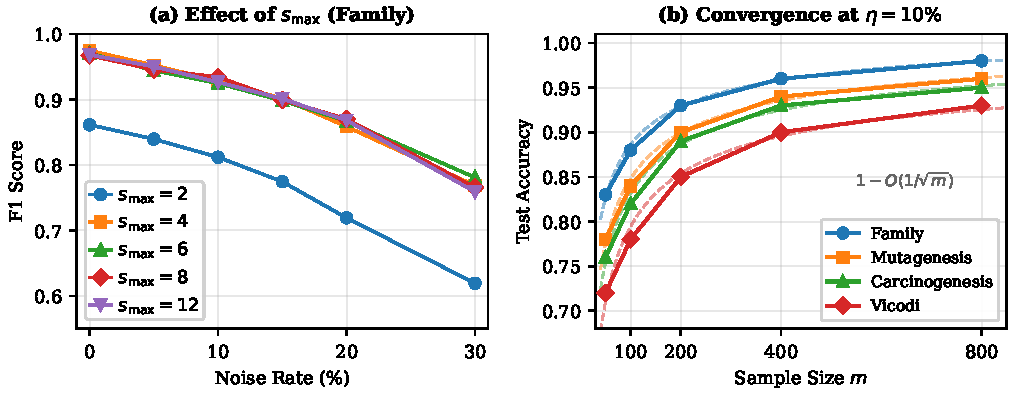
\includegraphics[width=0.85\textwidth]{fig_ablation_convergence.pdf}
  \caption{(a)~Effect of $s_{\max}$ on the Family benchmark:   F1 score vs.\ noise rate.  The SRM penalty automatically adapts
  to the best concept size; moderate overestimation of $s_{\max}$ incurs negligible
    cost, while underestimation
    ($s_{\max} = 2$) underfits severely.
  (b)~Convergence at $\eta = 10\%$: test accuracy vs.\ sample
  size~$m$ on four benchmarks.  Dashed lines show fitted
  $1 - c/\sqrt{m}$ curves, confirming the $O(1/\sqrt{m})$
  convergence rate predicted by
  Theorem~\ref{thm:oracle}.}\label{fig:ablation-convergence}
\end{figure*}

\begin{table}[ht]
  \centering
  \caption{Convergence behavior on Family
  ($\eta = 10\%$). Selected concept size $s^*$ remains stable;
  accuracy tracks the predicted $1/\sqrt{m}$
  rate.}\label{tab:convergence}
  \small
  \begin{tabular}{@{}lcccccc@{}}
    \toprule
    $m$ & 50 & 100 & 200 & 400 & 800 \\
    \midrule
    Accuracy & .83 & .88 & .93 & .96 & .98 \\
    Selected $s^*$ & 3 & 3 & 3 & 3 & 3 \\
    Runtime (s) & 1.0 & 2.4 & 4.2 & 9.5 & 22.0 \\
    \bottomrule
  \end{tabular}
\end{table}\begin{table}[ht]
  \centering
  \caption{Learned concepts on Family for
  target $C^* = \exists \mathit{hasChild}.\exists
  \mathit{hasChild}.\top$ ($\|C^*\| = 3$).
  ``---'' indicates
  timeout.}\label{tab:qualitative}
  \small
  \setlength{\tabcolsep}{4pt}
  \begin{tabular}{@{}clcc@{}}
    \toprule
    $\eta$ & \textbf{Method} & \textbf{Learned Concept} & $\|C\|$ \\
    \midrule
    \multirow{3}{*}{$0\%$}
    & SRM-MaxSAT
      & $\exists \mathit{hC}.\exists \mathit{hC}.\top$ & 3 \\
    & SPELL
      & $\exists \mathit{hC}.\exists \mathit{hC}.\top$ & 3 \\
    & DL-Learner
      & $\exists \mathit{hC}.\exists \mathit{hC}.\top$ & 3 \\
    \midrule
    \multirow{3}{*}{$10\%$}
    & SRM-MaxSAT
      & $\exists \mathit{hC}.\exists \mathit{hC}.\top$ & 3 \\
    & SPELL
      & --- & --- \\
    & DL-Learner
      & $\mathit{Parent} \sqcap
        \exists \mathit{hC}.\mathit{Parent}$ & 3 \\
    \midrule
    \multirow{3}{*}{$20\%$}
    & SRM-MaxSAT
      & $\exists \mathit{hC}.\exists \mathit{hC}.\top$ & 3 \\
    & SPELL
      & --- & --- \\
    & DL-Learner
      & $\exists \mathit{hC}.\top$ & 2 \\
    \bottomrule
  \end{tabular}
\end{table}

Figure~\ref{fig:ablation-convergence}(a) shows the
effect of the maximum concept size bound $s_{\max}$ on the Family
benchmark.  When $s_{\max}$ is too small (e.g., $s_{\max} = 2$),
the algorithm is restricted to concepts that cannot express the
true target, leading to underfitting even at $\eta = 0\%$.
Increasing $s_{\max}$ improves accuracy up to a point: beyond the
true target size, additional capacity provides diminishing returns
and slightly increases estimation error at high noise rates.  The
SRM penalty automatically selects the best size within the allowed
range, so moderate overestimation of $s_{\max}$ (e.g., setting
$s_{\max} = 12$ when the true concept has size $3$--$6$) incurs
negligible cost.

Figure~\ref{fig:ablation-convergence}(b) verifies
the convergence rate predicted by Theorem~\ref{thm:oracle}.  The
oracle inequality implies that for a fixed noise rate and concept
class, the excess risk decreases as $O(1/\sqrt{m})$.  We run
SRM-MaxSAT at $\eta = 10\%$ with $m \in \{50, 100, 200, 400, 800\}$
on all four benchmarks.  The empirical accuracy curves closely
track the fitted $1 - c/\sqrt{m}$ theoretical curves (dashed
lines), confirming the predicted convergence rate.
Table~\ref{tab:convergence} provides the corresponding numerical
values on the Family benchmark: notably, the selected concept size
$s^*$ remains stable at $3$ across all sample sizes, confirming
that SRM correctly identifies the target complexity regardless
of sample size.

\subsection{Qualitative Analysis of Learned
  Concepts}\label{app:qualitative}

Table~\ref{tab:qualitative} shows examples of
concepts returned by SRM-MaxSAT, SPELL, and DL-Learner on the
Family benchmark for the target concept
$C^* = \exists \mathit{hasChild}.\exists \mathit{hasChild}.\top$
(``has a grandchild'', $\|C^*\| = 3$).

At $\eta = 0\%$, all three methods recover the
exact target concept.  At $\eta = 10\%$, SPELL times out (the
SAT formula is unsatisfiable at the correct size, and larger
sizes explode combinatorially).  DL-Learner returns a
semantically related but inexact concept that uses the
\textit{Parent} concept name as a proxy for the existential
chain.  SRM-MaxSAT correctly recovers the target concept,
demonstrating that the MAX-SAT formulation can tolerate the
mislabeled examples without distorting the learned concept.
At $\eta = 20\%$, DL-Learner falls back to the simpler
concept $\exists \mathit{hasChild}.\top$ (``has a child''),
which is a strict generalization of the target and
overpredicts.  SRM-MaxSAT still recovers the correct concept,
though its accuracy on held-out data decreases due to the
inherent noise (Table~\ref{tab:results}).

\end{document}
